%% --------------------------------------------------------------------------
%%  Tese de Mestrado - Defesa Final
%%  Felipe Augusto Oliveira dos Santos
%%  Faculdade de Engenharia El\'{e}trica e de Computa\c{c}\~{a}o (FEEC)
%%  Universidade Estadual de Campinas (Unicamp)
%%
%%  Template: FEEC modelo tese (CCPG 001-2015) — abnTeX2-based.
%% --------------------------------------------------------------------------

\input{preambulo}

% --- compila o \'{\i}ndice  ---
\makeindex
% ---

% ---- In\'{\i}cio do documento ----
\begin{document}

% Retira espa\c{c}o extra obsoleto entre as frases.
\frenchspacing

% ============================================================================
% ELEMENTOS PR\'{E}-TEXTUAIS
% ============================================================================

% --- Capa ---
\imprimircapa

% --- Folha de rosto ---
\imprimirfolhaderosto

% --- Ficha catalogr\'{a}fica (placeholder) ---
\begin{fichacatalografica}
    \vspace*{\fill}
    \begin{center}
        \textsc{Inclua aqui o pdf com a ficha catalogr\'{a}fica fornecida pela BAE.}
    \end{center}
    \vspace*{\fill}
    %\includepdf{ficha-catalografica.pdf}
\end{fichacatalografica}

% --- Folha de aprova\c{c}\~{a}o (placeholder) ---
\newpage
\vspace*{\fill}
\begin{center}
    \textsc{Inclua aqui a folha de assinaturas.}
\end{center}
\vspace*{\fill}
\newpage
%\includepdf[pagecommand={\thispagestyle{plain}}]{folha-assinaturas.pdf}
\cleardoublepage

% --- Dedicat\'{o}ria ---
\begin{dedicatoria}
    \vspace*{\fill}
    \centering
    \noindent
    \textit{To my family.}
    \vspace*{\fill}
\end{dedicatoria}

% --- Agradecimentos ---
\begin{agradecimentos}
    I would like to thank my advisor, Prof.\ Dr.\ Denis Fantinato, for his
    continuous guidance, patience, and insight throughout this work. I am also
    grateful to the Faculdade de Engenharia El\'{e}trica e de Computa\c{c}\~{a}o
    (FEEC) at Unicamp for providing the environment in which this research
    was carried out, and to my colleagues and family for their unwavering
    support.
\end{agradecimentos}

% --- Resumo (PT) e Abstract (EN) ---
\begin{resumo}
A proliferação exponencial da Internet das Coisas (IoT) tem produzido uma vasta
rede de dispositivos interconectados, enquanto o impacto econômico global das
ameaças cibernéticas continua a crescer. As restrições computacionais e de
memória de muitos dispositivos IoT tornam ineficazes as soluções de segurança
tradicionais e motivam mecanismos de defesa adaptativos capazes de operar
autonomamente. Esta dissertação propõe e avalia rigorosamente um arcabouço de
defesa adaptativo para redes IoT que combina predição proativa de ataques com
Aprendizado por Reforço Profundo (DRL). O sistema é avaliado no \emph{dataset}
CICIoT2023, projetado sobre uma cadeia de eliminação cibernética (Cyber Kill
Chain) de cinco estágios, com um gerador LSTM, um detector de estágio supervisionado
e um ambiente Gymnasium customizado expondo um agente defensor com cinco ações.
Três algoritmos DRL (DQN, PPO, A2C) são treinados ao longo de dez sementes e
comparados a quatro políticas de referência e a um oráculo. O melhor agente
implantável (PPO) captura 81\,\% do teto do oráculo com uma vantagem de latência
de 141$\times$ sobre a baseline supervisionada mais forte, e todos os resultados
são reprodut\'{\i}veis por uma cadeia de \emph{hashes} SHA-256 verificada de ponta a
ponta.

    \vspace{\onelineskip}

    \noindent\textbf{Palavras-chaves}: Segurança IoT; Aprendizado por Reforço Profundo;
    Cyber Kill Chain; Predição de Estágio de Ataque; LSTM; CICIoT2023; Reprodutibilidade.

    \vspace{\onelineskip}
    \vspace{\onelineskip}

    \begin{otherlanguage*}{english}
    \begin{center}{\ABNTEXchapterfont\huge Abstract}\end{center}

The exponential proliferation of the Internet of Things (IoT) has produced a
vast network of interconnected devices while the global economic impact of cyber
threats continues to grow. The computational and memory constraints of many IoT
devices render traditional security solutions ineffective and motivate
intelligent, adaptive defence mechanisms capable of operating autonomously.
This dissertation designs, implements, and rigorously evaluates an adaptive
defence framework for IoT networks that combines proactive attack-stage
prediction with Deep Reinforcement Learning (DRL). The framework is evaluated
end-to-end on the CICIoT2023 dataset, projected onto a five-stage Cyber Kill
Chain, with an LSTM red-team generator, a supervised stage detector, and a
custom Gymnasium environment exposing a five-action defender. Three DRL
algorithms (DQN, PPO, A2C) are trained over ten seeds and benchmarked against
four reference policies and an oracle. The best deployable agent (PPO)
captures 81\,\% of the oracle ceiling at a 141$\times$ latency advantage over
the strongest supervised baseline, and every reported number is reproducible
from a SHA-256 hash chain verified end-to-end.

    \vspace{\onelineskip}

    \noindent\textbf{Keywords}: IoT security; Deep Reinforcement Learning; Cyber
    Kill Chain; Attack Stage Prediction; LSTM; CICIoT2023; Reproducibility.

    \end{otherlanguage*}
\end{resumo}

% --- Listas (figuras, tabelas, ToC) ---
\pdfbookmark[0]{\listfigurename}{lof}
\listoffigures*
\cleardoublepage

\pdfbookmark[0]{\listtablename}{lot}
\listoftables*
\cleardoublepage

\pdfbookmark[0]{\contentsname}{toc}
\tableofcontents*
\clearpage

% ============================================================================
% ELEMENTOS TEXTUAIS
% ============================================================================
\pagenumbering{arabic}
\setcounter{page}{1}

\textual

% ===============================================================
% Chapter 1 — Introduction
% ===============================================================
\chapter{Introduction}\label{cap:intro}

% --- Section 1.1 ---
\section{The Case for Adaptive IoT Security}\label{sec:case_for_adaptive_security}
The Internet of Things (IoT) connects billions of embedded devices --- smart cameras, industrial sensors, medical monitors, and home appliances --- into a single, globally addressable network. The number of IoT devices worldwide is forecast to more than double from 19.8 billion in 2025 to over 40.6 billion by 2034 \cite{Statista2025}, an exponential growth that has produced a vast and multifaceted attack surface. The financial ramifications are staggering: global damages from cybercrime are projected to reach USD 12.2 trillion annually by 2031 \cite{Morgan2025}. Malicious actors increasingly exploit insecure devices to steal data, disrupt services, or form large-scale botnets for Distributed Denial of Service (DDoS) attacks \cite{Neto2023,Tawalbeh2020}.

Securing this landscape presents unique and formidable challenges that render traditional IT security paradigms insufficient. First, most IoT devices are severely \textbf{resource-constrained}, possessing minimal computational power, memory, and energy, which precludes the use of intensive security software like traditional firewalls or antivirus agents \cite{Chen2021}. Second, IoT ecosystems are defined by extreme \textbf{heterogeneity}, comprising countless devices using disparate protocols and operating systems, which makes uniform security policy enforcement nearly impossible \cite{Mavroeidis2023}. This complexity is amplified by the large-scale, dynamic nature of these networks and the physical vulnerability of devices often deployed in unsecured locations \cite{AlGaradi2020}.

Consequently, conventional security tools are fundamentally ill-equipped for this environment. \textbf{Signature-based Intrusion Detection Systems (IDS)}, the cornerstone of many legacy systems, rely on static databases of known attack patterns. This approach is purely reactive and fails against novel or \textbf{zero-day attacks} --- threats for which no signature yet exists \cite{Khraisat2019,Yang2024}. While \textbf{anomaly-based IDS} attempt to overcome this by baselining ``normal'' behaviour, the dynamic and heterogeneous nature of IoT traffic makes establishing a reliable baseline exceptionally difficult, leading to high \textbf{false positive rates} that can disrupt critical functions \cite{Ibitoye2021,Tharewal2022}.

The core limitation of these paradigms is their lack of adaptability. They are built on static models and cannot autonomously evolve. This creates a critical need for a new security paradigm: one that is forward-looking, data-driven, and capable of autonomous decision-making. \textbf{Deep Reinforcement Learning (DRL)}, a field of machine learning focused on goal-oriented learning from interaction, has emerged as a powerful framework for such a system \cite{Chen2021}. A DRL agent learns an optimal decision-making strategy, or \textbf{policy}, through trial-and-error interaction with its environment. Unlike static systems, a DRL agent can generalise from its experience to respond to novel threats and can adapt its policy as new adversarial tactics emerge, making it well-suited for the non-stationary nature of IoT security \cite{Sutton2018,Uprety2021}. By framing cyber-defense as a sequential decision-making problem, DRL provides a robust mathematical foundation for creating autonomous security systems that can learn to outmaneuver attackers \cite{Gueriani2023}.

% --- Section 1.2 ---
\section{Problem Statement and Contributions}\label{sec:proposal_and_contributions}
The preceding analysis culminates in a clear research problem: existing IoT security frameworks are not simultaneously \textbf{adaptive}, \textbf{data-driven}, and \textbf{rigorously benchmarked} against deployable reference policies under a unified evaluation contract. Reactive signature-based systems cannot generalise to novel attacks, supervised classifiers do not act, and prior DRL-for-IoT work seldom reports head-to-head comparisons against the full set of deployable baselines a security operator has at hand --- random, always-block, and a supervised stage classifier composed with a recommended-action mapping.

This dissertation directly addresses that gap by designing, implementing, and rigorously evaluating a closed-loop adaptive defense framework for IoT networks that combines LSTM-based kill-chain stage modeling with Deep Reinforcement Learning, validated end-to-end on the contemporary CICIoT2023 dataset. Concretely, this work makes the following contributions:

\begin{enumerate}
    \item \textbf{A kill-chain-aware adaptive defense framework.} A two-stage architecture combining (i) a Long Short-Term Memory (LSTM) red-team episode generator trained on stage-labelled CICIoT2023 sequences, which drives a \texttt{RealisationEngine} that samples real feature rows per kill-chain stage, with (ii) a custom Gymnasium environment exposing a five-action defender (observe, log, throttle, block, isolate) under a stage-action proportionality reward inspired by the IoTWarden recommended-action mapping~\cite{Alam2024}. The attacker model is bounded by a \textbf{monotonic-attacker assumption}: the LSTM generates upper-triangular stage transitions in which the kill chain advances but never retreats. The framework is developed and validated on the \textbf{CICIoT2023 dataset}~\cite{Neto2023}, projected onto a five-stage Cyber Kill Chain (benign, recon, access, maneuver, impact) with a documented per-class mapping, with out-of-distribution classes held out disjointly from training.

    \item \textbf{A reward-mis-specification analysis for kill-chain-aware RL.} A naive contract that terminates the episode at the first \textsc{impact} step ({\small\texttt{impact\_is\_terminal=True}}) causes the agent to learn a cocked-trigger strategy that scores deceptively high on validation but fails to achieve genuine threat mitigation at benchmark scale. Identifying and correcting this mis-specification --- by allowing the agent one additional decision turn after \textsc{impact} ({\small\texttt{impact\_is\_terminal=False}}) --- is a primary contribution of this work. The corrected primary contract is the basis for all reported benchmark numbers.

    \item \textbf{A comparative DRL benchmark with a ${\sim}146{\times}$ latency advantage over the supervised deployable baseline.} DQN, PPO, and A2C are trained over ten seeds under the primary contract and evaluated on a held-out balanced test split (300 episodes per policy) against four reference policies: random, always-observe, always-block, and a supervised RandomForest stage classifier composed with the recommended-action mapping (RF-Acting). A rule-based policy with free access to the true attack stage is reported as an \emph{oracle ceiling} (\OracleCeiling{}). The best deployable trained agent (A2C, \BestAgentReward{}) captures \textbf{\OracleCapturePct{}\,\%} of that ceiling with non-overlapping bootstrap confidence intervals against every non-RL baseline. Among deployable policies the comparison is a latency--reward trade-off: trained RL agents achieve inference at ${\sim}0.095$\,ms per decision versus RF-Acting at 13.83\,ms --- a ${\sim}146{\times}$ advantage --- at a reward cost of approximately 10\,\%. A caveat applies: the best-reward trained agent (A2C) also carries the highest benign false-positive rate (11.5\,\%), while DQN offers a lower-FPR operating point (6.1\,\%) at marginally lower reward.

    \item \textbf{Reward-component and out-of-distribution ablations.} A 12-cell sparse one-at-a-time sweep over five reward coefficients $\times$ $\{0.5\times, 1\times, 2\times\}$ plus the binary termination-contract flag characterises the reward landscape. No single linear perturbation closes the residual gap; the structural \texttt{impact\_is\_terminal} change is the highest-impact lever, which in an ablation probe (PPO-only, $n=30$ episodes) raises the mitigated-impact rate from 0.153 to 0.840. At full benchmark scale ($n=300$, 10 seeds) the primary-contract agents achieve mitigated-impact rates of 0.26--0.32, a genuine improvement over the mis-specified baseline (0.153). A separate evaluation against four held-out out-of-distribution attack classes yields the pre-registered finding that the trained policy is \emph{robust to}, but not better at, the class on which the supervised stage detector is structurally blind (recall\,$=\,0.001$).

    \item \textbf{An audit-first reproducibility protocol.} Every figure ships a \texttt{manifest.json} that pins the SHA-256 hashes of every input artefact (data splits, trained models, scaler, episode roll-outs) and the producing Git commit. All results are reproducible via a SHA-256-verified artifact chain. The protocol is documented in Appendix~\ref{app:repro}.
\end{enumerate}

The remainder of this dissertation is structured as follows. Chapter~\ref{cap:background} provides a detailed review of background concepts in IoT security, the Cyber Kill Chain, and reinforcement learning, and situates this work against related research. Chapter~\ref{cap:methodology} details the proposed framework architecture, including the kill-chain projection of CICIoT2023, the LSTM red team and stage detector, the Markov Decision Process underlying the environment, the reward function, the training protocol, and the baseline policies. Chapter~\ref{cap:results} presents the empirical results across all phases of the pipeline and discusses the headline findings, including the oracle-ceiling reframe, the reward-component ablation, and the out-of-distribution robustness story. Chapter~\ref{cap:conclusion} summarises the contributions, discusses limitations and threats to validity, and outlines future work.

% ====================================================================
% Section: Background and Related Work (Revised)
% ====================================================================
\section{Background and Related Work}\label{sec:background}

This section establishes the theoretical groundwork and contextualizes the contributions of this thesis. Section \ref{subsec:rl_concepts} first introduces the foundational principles of Reinforcement Learning (RL) and the specific Deep Reinforcement Learning (DRL) algorithms central to this work. Section \ref{subsec:related_work_iot} then provides a review of related research in IoT security, situating this project within the broader academic landscape and highlighting its novel contributions.

% --- Subsection 2.1 ---
\subsection{Reinforcement Learning for Autonomous Systems}\label{subsec:rl_concepts}
Reinforcement Learning is a computational paradigm focused on goal-directed learning from interaction. An intelligent agent learns to make optimal decisions not by being shown labeled examples, but by exploring an environment and discovering which sequences of actions yield the greatest cumulative reward \cite{Sutton2018}. This learning process is formalized through the mathematical framework of Markov Decision Processes (MDPs).

\subsubsection{Markov Decision Processes}\label{subsubsec:mdp}
An MDP provides a formal model for sequential decision-making under uncertainty. The core principle is the \textbf{Markov Property}, which asserts that the current state provides all necessary information to make an optimal decision, rendering the history of prior states irrelevant \cite{Sutton2018}. An MDP is defined as a five-tuple $(S, A, P, R, \gamma)$:
\begin{itemize}
    \item \textbf{S}: A finite set of states, representing all possible configurations of the environment. In this thesis, a state $s \in S$ is a complex observation composed of current network traffic features, a history of recent states and actions, and predictions from the LSTM attack model.
    \item \textbf{A}: A finite set of actions. For this work, $A$ consists of four discrete defensive actions: \{`monitor`, `rate-limit`, `block IP`, `shutdown service`\}.
    \item \textbf{P}: The state transition probability function, $P(s' | s, a) = P(S_{t+1}=s' | S_t=s, A_t=a)$, defining the dynamics of the environment.
    \item \textbf{R}: The reward function, $R(s, a, s')$, which provides the immediate numerical feedback for transitioning from $s$ to $s'$ via action $a$.
    \item \textbf{$\gamma$}: The discount factor ($0 \leq \gamma \leq 1$), which prioritizes immediate rewards over future ones.
\end{itemize}
The agent's objective is to learn a \textbf{policy}, $\pi(a|s)$, which maps states to a probability distribution over actions, to maximize the expected discounted return.

\subsubsection{Value Functions and Bellman Equations}\label{subsubsec:bellman}
To determine the quality of states and actions, RL uses value functions. The \textbf{state-value function}, $V^\pi(s)$, is the expected return from state $s$ while following policy $\pi$:
\begin{equation}\label{eq:state_value_function}
V^\pi(s) = \mathbb{E}_\pi \left[ \sum_{k=0}^{\infty} \gamma^k R_{t+k+1} \Big| S_t = s \right]
\end{equation}
The \textbf{action-value function} (or Q-function), $Q^\pi(s, a)$, is the expected return after taking action $a$ from state $s$ and then following policy $\pi$:
\begin{equation}\label{eq:action_value_function}
Q^\pi(s,a) = \mathbb{E}_\pi \left[ \sum_{k=0}^{\infty} \gamma^k R_{t+k+1} \Big| S_t = s, A_t = a \right]
\end{equation}
These functions adhere to the recursive relationships defined by the Bellman equations. The \textbf{Bellman optimality equation} for the Q-function is central to many RL algorithms and is expressed as:
\begin{equation}\label{eq:bellman_optimality}
Q^*(s, a) = \mathbb{E}_{s' \sim P(\cdot|s,a)} \left[ R(s,a,s') + \gamma \max_{a' \in A} Q^*(s', a') \right]
\end{equation}
Solving this equation yields the optimal Q-function, $Q^*(s, a)$, from which the optimal policy can be derived by selecting the action with the highest value in each state.

\subsubsection{Deep Reinforcement Learning Algorithms}\label{subsubsec:drl_algorithms}
For environments with large or continuous state spaces, like an IoT network, tabular methods are intractable. Deep Reinforcement Learning (DRL) overcomes this by using deep neural networks to approximate the value functions or policies \cite{Chen2021}. This thesis implements and benchmarks three seminal DRL algorithms that represent the primary families of RL.

\paragraph{Deep Q-Networks (DQN)}
DQN is a value-based algorithm that uses a neural network to approximate the action-value function, $Q(s, a; \theta) \approx Q^*(s, a)$ \cite{Mnih2015}. To stabilize learning, DQN introduces two critical mechanisms:
\begin{itemize}
    \item \textbf{Experience Replay:} Experiences $(s_t, a_t, r_t, s_{t+1})$ are stored in a large replay buffer. The network is trained on mini-batches randomly sampled from this buffer, which breaks temporal correlations in the data.
    \item \textbf{Fixed Target Network:} A separate, periodically updated target network is used to generate stable target values for the Bellman equation, preventing oscillations during training. The loss function is typically the Mean Squared Bellman Error (MSBE):
    \begin{equation}\label{eq:dqn_loss}
    L(\theta) = \mathbb{E}_{(s,a,r,s') \sim D} \left[ \left( \underbrace{(r + \gamma \max_{a'} Q(s', a'; \theta^-))}_{\text{Target Q-value}} - \underbrace{Q(s, a; \theta)}_{\text{Predicted Q-value}} \right)^2 \right]
    \end{equation}
    where $\theta^-$ are the parameters of the fixed target network.
\end{itemize}

\paragraph{Proximal Policy Optimization (PPO)}
PPO is a state-of-the-art actor-critic algorithm that directly optimizes a parameterized policy (the actor) while using a value function (the critic) to reduce variance \cite{Schulman2017}. Its key innovation is a clipped surrogate objective function that constrains the size of policy updates, ensuring greater training stability. The objective function is:
\begin{equation}\label{eq:ppo_clip}
L^{CLIP}(\theta) = \hat{\mathbb{E}}_t \left[ \min \left( r_t(\theta)\hat{A}_t, \text{clip}(r_t(\theta), 1-\epsilon, 1+\epsilon)\hat{A}_t \right) \right]
\end{equation}
where $r_t(\theta)$ is the probability ratio between the new and old policies, $\hat{A}_t$ is the estimated advantage, and $\epsilon$ is a hyperparameter that constrains the policy change. This approach prevents destructive policy updates and is known for its reliability and performance.

\paragraph{Advantage Actor-Critic (A2C)}
A2C is a synchronous variant of the foundational Asynchronous Advantage Actor-Critic (A3C) algorithm \cite{Mnih2016}. Like PPO, it is an actor-critic method, but it uses a simpler, unconstrained policy update mechanism. It typically employs multiple parallel workers to collect experience simultaneously. These experiences are then aggregated to compute a single, stable gradient update for both the actor (policy) and the critic (value function). While often faster to converge than PPO on simpler problems, it can be less stable.

All three algorithms are implemented in this thesis using Stable Baselines3's `MultiInputPolicy`, which is designed to handle the `Dict` observation space provided by our custom IoT environment.

% --- Subsection 2.2 ---
\subsection{Related Work in AI-Driven IoT Security}\label{subsec:related_work_iot}
The application of artificial intelligence to IoT security is an active and rapidly evolving field of research. Early work focused on applying classical machine learning models to intrusion detection, which has since paved the way for more sophisticated, adaptive systems based on Deep Reinforcement Learning.

\subsubsection{Machine Learning Approaches for Intrusion Detection}
Early approaches to intelligent IoT security leveraged supervised and unsupervised machine learning for building Intrusion Detection Systems (IDS). Supervised models, such as Support Vector Machines (SVM) and Random Forests, were trained on labeled datasets to classify network flows as either benign or malicious \cite{AlGaradi2020}. While effective at identifying known attack patterns, these models struggle with novel or \textbf{zero-day attacks} not seen during training, a limitation they share with traditional signature-based IDS \cite{Khraisat2019}. Furthermore, they typically operate as passive classifiers, identifying threats without the capacity for automated, sequential defensive actions.

\subsubsection{The Shift to Active Defense with DRL}
The limitations of static ML models motivated a shift towards DRL to create autonomous agents capable of active, closed-loop cyber-defense. Several notable works have explored this domain, providing a foundation upon which this thesis builds.

Some research has focused on using RL for deception and intelligence gathering. The work of Guan et al. (2023) in \textbf{HoneyIoT}, for example, presents an adaptive high-interaction honeypot that uses RL to learn an attacker's behavior and dynamically alter its services to keep the attacker engaged and reveal their methods \cite{Guan2023}. While this is a powerful application of RL, its primary purpose is reconnaissance, whereas our system is designed as a direct defense mechanism for a live network.

Other works have targeted specific layers of the IoT ecosystem. \textbf{IoTWarden}, proposed by Alam et al. (2024), uses a DQN agent to mitigate attacks in trigger-action IoT platforms (like IFTTT) by identifying and disabling malicious rules or "applets" in real-time \cite{Alam2024}. This approach is highly effective for its targeted domain but is confined to the application layer. Similarly, the work by Nguyen et al. (2021) proposes a Federated DRL system for traffic monitoring in Software-Defined Networks (SDN) for IoT, focusing on efficient data collection and analysis rather than active defense \cite{Nguyen2021}. Our research addresses a more fundamental challenge by operating at the \textbf{network layer}, analyzing features derived from raw traffic to defend against a broad range of network-level attacks such as DDoS, DoS, and Spoofing, which are prevalent in the CICIoT2023 dataset.

\subsubsection{Positioning the Thesis: Bridging the Research Gap}
While previous works have successfully applied DRL to specific aspects of IoT security, a gap remains for a comprehensive, network-level defense system that is simultaneously:
\begin{itemize}
    \item \textbf{Proactive and Adaptive:} Uniquely combining a data-driven predictive model (an LSTM) with a DRL-based agent to create a closed loop from threat anticipation to autonomous action.
    \item \textbf{Grounded in Realistic, Modern Data:} Validated on the large-scale and contemporary \textbf{CICIoT2023 dataset}, ensuring that the learned policies are relevant to modern, real-world attack vectors.
    \item \textbf{Network-Layer Focused:} Designed to defend against a broad range of fundamental network attacks by analyzing traffic-flow features.
    \item \textbf{Rigorously Benchmarked:} Providing a thorough, empirical comparison of modern value-based (DQN) and actor-critic (PPO, A2C) algorithms for this specific proactive defense task.
\end{itemize}
This thesis directly addresses this gap by designing, implementing, and evaluating a complete framework that integrates these critical components, thereby advancing the development of resilient, intelligent systems capable of defending the vast and ever-expanding IoT landscape.
% ====================================================================
% Section: Proposed Methodology (Revised)
% ====================================================================
\section{Methodology}\label{sec:methodology}

This section details the methodology employed to design, implement, and evaluate the proposed adaptive IoT defense system. The framework is architected as a multi-stage, closed-loop process that synergizes predictive modeling with autonomous decision-making to create a proactive security posture. Section \ref{subsec:framework_architecture} provides a high-level overview of this architecture. Section \ref{subsec:data_source} describes the real-world dataset and preprocessing pipeline that form the empirical foundation of the system. The subsequent sections detail the design of the proactive attack prediction module (Section \ref{subsec:lstm_module}), the reinforcement learning environment (Section \ref{subsec:rl_environment}), and the training and benchmarking of the DRL defense agents (Section \ref{subsec:drl_training}).

% --- Subsection 3.1 ---
\subsection{Framework Architecture Overview}\label{subsec:framework_architecture}
The proposed framework is designed to transition IoT security from a reactive to a proactive paradigm. This is achieved through the architecture illustrated in Figure \ref{fig:framework_overview}, which can be understood through three primary stages.

\begin{figure}[h!]
    \centering
    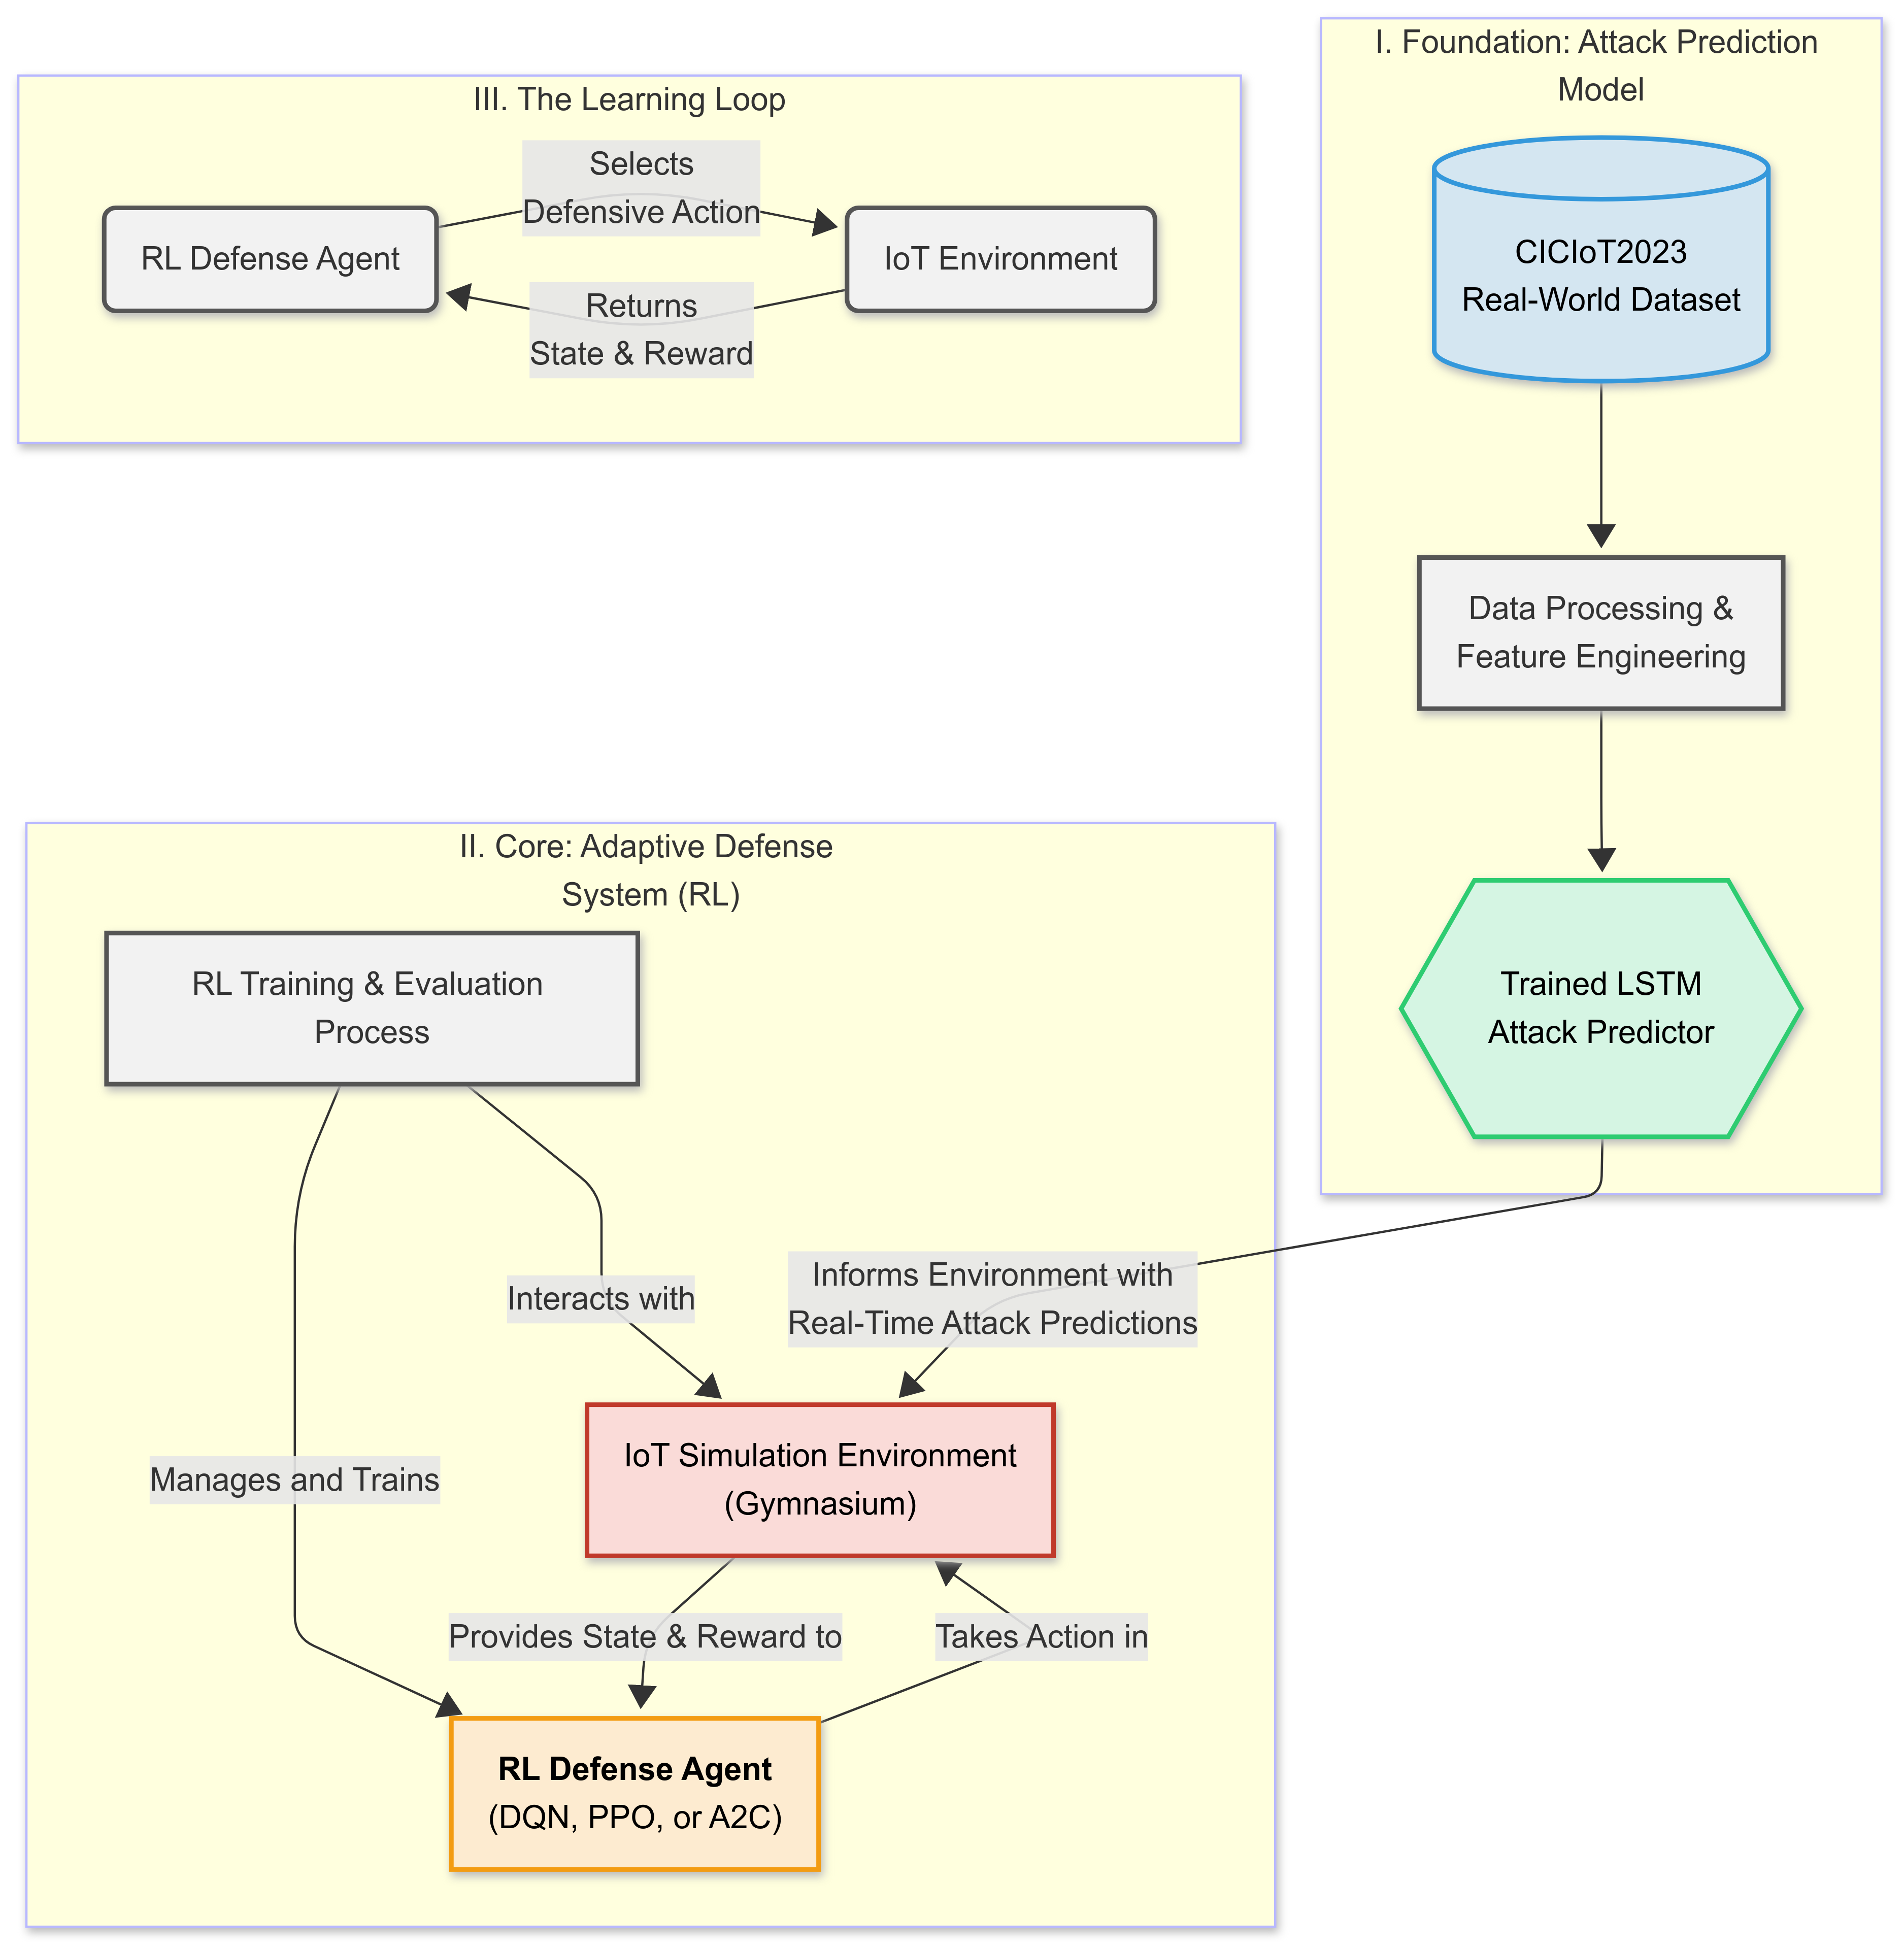
\includegraphics[width=0.85\textwidth]{figs/iot_rl_defense_system_diagram_mermaid.png}
    \caption{High-Level Architecture of the Proactive-Adaptive Defense System.}
    \label{fig:framework_overview}
\end{figure}

The three stages are:
\begin{enumerate}
    \item \textbf{Stage I: Predictive Foundation.} In this initial, offline stage, a Long Short-Term Memory (LSTM) based neural network is trained on a comprehensive, real-world IoT dataset. The objective is to develop a robust predictive model capable of identifying temporal patterns in network traffic that are indicative of imminent or ongoing cyberattacks. This pre-trained model serves as the system's "intelligence core," providing proactive threat assessments.
    
    \item \textbf{Stage II: Core Adaptive Defense System.} The second stage involves the primary training process for the defense agent. A DRL agent is trained within a custom-built simulation environment that models an IoT network. Crucially, this environment is informed by the predictions of the LSTM model from Stage I, which are integrated directly into the agent's observations.
    
    \item \textbf{Stage III: The Learning Loop.} This stage represents the fundamental reinforcement learning cycle that governs the adaptive defense system in Stage II. At each step of the simulation, the RL agent selects a defensive action, which is applied to the IoT environment. The environment, in turn, returns a new state and a corresponding reward signal. This continuous feedback loop is the mechanism through which the agent learns an optimal defense policy via trial and error.
\end{enumerate}
This decoupled architecture allows the system to ground its understanding of threats in real-world data (Stage I) while learning to apply that understanding to execute effective, autonomous defensive maneuvers through a formal learning process (Stages II and III).

% --- Subsection 3.2 ---
\subsection{Data Source and Preprocessing}\label{subsec:data_source}
The empirical validity of any AI-driven security system is fundamentally dependent on the quality and realism of its training data. This research utilizes the \textbf{CICIoT2023 dataset}, a contemporary and extensive resource for IoT security research \cite{Neto2023}.

\subsubsection{The CICIoT2023 Dataset}\label{subsubsec:dataset_desc}
The CICIoT2023 dataset was developed by the Canadian Institute for Cybersecurity (CIC) to address the need for a realistic benchmark reflecting modern IoT network traffic. Its key characteristics make it uniquely suited for this work:
\begin{itemize}
    \item \textbf{Realistic Testbed:} The data was captured from a physical topology of 105 real IoT devices, including smart cameras, speakers, sensors, and hubs \cite{Neto2023}.
    \item \textbf{Comprehensive Attack Coverage:} It contains benign traffic alongside labeled data for 33 distinct attack types, which are grouped into seven major categories: DDoS, DoS, Reconnaissance, Web-based, Brute Force, Spoofing, and Mirai variants \cite{Neto2023}.
    \item \textbf{Modern Attack Vectors:} A key feature of the dataset is that attacks were executed \textit{by} other compromised IoT devices within the testbed, simulating realistic botnet and device-to-device attack scenarios \cite{Neto2023}.
\end{itemize}

%\subsubsection{Data Preprocessing Pipeline}\label{subsubsec:preprocessing}
%To prepare the dataset for model training, a multi-step preprocessing pipeline was implemented. The raw network flow data, provided in CSV format, undergoes the following transformations:
%\begin{enumerate}
%    \item \textbf{Data Cleaning:} Rows with missing or infinite values are removed to ensure data integrity.
%    \item \textbf{Feature Scaling:} All numerical features are standardized using a `StandardScaler`. This process removes the mean and scales the data to unit variance, which is critical for the stable training of neural networks.
%    \item \textbf{Label Encoding:} The categorical attack labels are converted into a numerical format using a `LabelEncoder`.
%    \item \textbf{Data Splitting:} The dataset is divided into training (70\%), validation (15\%), and test (15\%) sets to ensure robust model evaluation and prevent overfitting.
%    \item \textbf{Sequence Generation:} For the LSTM model, the time-series data is transformed into sequences of a fixed length. Each sequence consists of a series of consecutive network flow feature vectors, with the label corresponding to the final time step in the sequence.
%\end{enumerate}
%The scaler and label encoder from this process are saved as artifacts to ensure consistent data transformation during both training and inference.

% --- Subsection 3.3 ---
\subsection{Proactive Attack Prediction Module}\label{subsec:lstm_module}
The proactive core of the framework is the attack prediction module, which is implemented as a Long Short-Term Memory (LSTM) network. LSTMs are a type of Recurrent Neural Network (RNN) specifically designed to learn long-term dependencies in sequential data, making them highly effective for time-series analysis of network traffic \cite{Hochreiter1997}.

\subsubsection{LSTM Model Architecture}
The attack prediction model consists of the following layers:
\begin{itemize}
    \item An \textbf{LSTM layer} that processes the input sequences of network features to capture temporal patterns.
    \item A \textbf{Dropout layer} for regularization to prevent overfitting.
    \item A series of \textbf{Fully Connected (Dense) layers} with ReLU activation functions to process the output from the LSTM layer.
    \item A final \textbf{Softmax output layer} that produces a probability distribution over all possible attack classes (including benign), representing the model's prediction.
\end{itemize}
The model is trained using the Adam optimizer and the Cross-Entropy Loss function, which are standard for multi-class classification tasks. The training process aims to minimize this loss, thereby learning an accurate mapping from a sequence of network data to a specific attack label.

% --- Subsection 3.4 ---
\subsection{Reinforcement Learning Environment Design}\label{subsec:rl_environment}
To train the DRL agents, a custom simulation environment was developed using the Gymnasium toolkit. This environment models the MDP described in Section \ref{subsubsec:mdp} and serves as the interactive training ground for the defense agents. Its core components are the state space, action space, and reward function.

\subsubsection{State and Action Spaces}
The environment is defined by a `Dict` observation space to provide the agent with a rich, multi-faceted view of the network's status.
\begin{itemize}
    \item \textbf{State Space ($S$):} The observation given to the agent at each timestep is a dictionary containing:
    \begin{itemize}
        \item \texttt{current\_state}: A vector of real-time network telemetry features.
        \item \texttt{state\_history}: A matrix containing a history of the last $N$ network states, allowing the agent to perceive temporal trends.
        \item \texttt{action\_history}: A vector of the last $M$ actions taken by the agent, providing it with self-awareness of its recent behavior.
        \item \texttt{attack\_prediction}: A vector of probabilities from the pre-trained LSTM model, representing the proactive assessment of the current threat level. This is the key link between the predictive and adaptive stages of the framework.
    \end{itemize}
    \item \textbf{Action Space ($A$):} The agent can select one of four discrete defensive actions:
    \begin{enumerate}
        \item \textbf{Monitor:} Take no action and continue observing.
        \item \textbf{Rate-Limit:} Restrict the traffic flow from suspicious sources.
        \item \textbf{Block IP:} Completely block traffic from identified malicious IPs.
        \item \textbf{Shutdown Service:} Temporarily disable a non-essential service under severe attack.
    \end{enumerate}
\end{itemize}

\subsubsection{Reward Function}
The design of the reward function is critical for guiding the agent toward the desired security posture. The function is engineered to balance threat mitigation with operational continuity. The composite reward at each timestep $t$, denoted $R_t$, is calculated as the sum of a prediction-based reward ($R_{pred}$) and an action-based reward ($R_{action}$):
$$ R_t = R_{pred} + R_{action} $$
Let $y_t \in \{0, 1\}$ be the true state of the network at timestep $t$ (where $1$ signifies an attack and $0$ signifies benign traffic), let $\hat{y}_t \in \{0, 1\}$ be the LSTM model's prediction, and let $\rho_t$ be the predicted risk score. The components are defined as follows:

\begin{itemize}
    \item \textbf{Prediction Reward ($R_{pred}$):} This component provides feedback based on the correctness of the LSTM's threat assessment. The reward is scaled by the model's confidence ($\rho_t$):
    \begin{equation}
    R_{pred} = 
    \begin{cases} 
        +10 \cdot \rho_t & \text{if } y_t=1 \text{ and } \hat{y}_t=1 \text{ (True Positive)} \\
        +5.0 & \text{if } y_t=0 \text{ and } \hat{y}_t=0 \text{ (True Negative)} \\
        -15 \cdot \rho_t & \text{if } y_t=1 \text{ and } \hat{y}_t=0 \text{ (False Negative)} \\
        -5 \cdot (1 - \rho_t) & \text{if } y_t=0 \text{ and } \hat{y}_t=1 \text{ (False Positive)}
    \end{cases}
    \end{equation}

    \item \textbf{Action Reward ($R_{action}$):} This component evaluates the suitability of the agent's action $a_t$ given the true state of the network. Actions are rewarded for effective mitigation during an attack and penalized for unnecessary disruption during benign traffic. Let $E(a_t)$ be an action's effectiveness bonus and $C(a_t)$ be its disruption cost, defined as:
    \begin{itemize}
        \item Action Effectiveness $E(a_t)$: Bonus values of $\{0.8, 0.9, 0.7, 0.6\}$ for actions \{`monitor`, `rate-limit`, `block IP`, `shutdown service`\}, respectively.
        \item Action Cost $C(a_t)$: Penalty values of $\{0.0, -1.0, -2.0, -3.0\}$ for the same actions.
    \end{itemize}
    The action reward is then:
    \begin{equation}
    R_{action} = 
    \begin{cases} 
        +5 \cdot E(a_t) & \text{if } y_t=1 \text{ (Attack ongoing)} \\
        C(a_t) & \text{if } y_t=0 \text{ (Benign traffic)}
    \end{cases}
    \end{equation}
\end{itemize}
This composite structure incentivizes the agent to learn a nuanced policy that trusts the predictor but also considers the operational impact of its actions, thereby balancing security with service continuity.

% --- Subsection 3.5 ---
\subsection{DRL Agent Training and Benchmarking}\label{subsec:drl_training}
The final component of the methodology is the training and evaluation of the DRL defense agents. To ensure robust and reproducible results, this work leverages the Stable Baselines3 library, a standard for high-quality DRL algorithm implementations.

\paragraph{Algorithm Selection}
Three prominent DRL algorithms were chosen to benchmark performance across different learning paradigms:
\begin{enumerate}
    \item \textbf{Deep Q-Network (DQN):} A classic value-based, off-policy algorithm that excels in discrete action spaces and serves as a strong baseline \cite{Mnih2015}.
    \item \textbf{Proximal Policy Optimization (PPO):} A state-of-the-art on-policy, actor-critic algorithm known for its stability and reliable performance \cite{Schulman2017}.
    \item \textbf{Advantage Actor-Critic (A2C):} A synchronous, on-policy actor-critic method that is often faster than PPO and provides another point of comparison \cite{Mnih2016}.
\end{enumerate}
All agents use a `MultiInputPolicy` architecture, which is specifically designed to process the `Dict` observation space from the custom IoT environment.
% ====================================================================
% Section: Results and Discussion
% ====================================================================
\clearpage
\chapter{Results and Discussion}\label{cap:results}

This chapter presents the empirical results across all stages of the framework. Section~\ref{sec:exp_setup} fixes the experimental setup. Section~\ref{sec:dataset_results} reports the kill-chain projection of CICIoT2023 and the splits-protocol audit (including the leakage-bug fix). Section~\ref{sec:red_team_results} validates the LSTM red-team episode generator; Section~\ref{sec:detector_results} validates the supervised stage detector. Section~\ref{sec:blue_team_results} reports the DRL training results, and Section~\ref{sec:benchmark_results} the held-out benchmarks against deployable baselines and the oracle reference. Section~\ref{sec:ablation_results} reports the reward-component and aggressiveness ablations, and Section~\ref{sec:ood_results} the out-of-distribution robustness evaluation. Section~\ref{sec:discussion} discusses the headline findings and threats to validity.

% --- Subsection 4.0 ---
\section{Experimental Setup}\label{sec:exp_setup}
The experiments were run on a single CPU core (no GPU is required for any development stage) using Python 3.9, PyTorch for the LSTM red-team and the stage detector, scikit-learn for the RandomForest baseline, Stable Baselines3 for the DRL agents, and Gymnasium for the custom environment. The blue-team training sweep (30 runs, 10 seeds $\times$ 3 algorithms) takes approximately 7.7 hours; the held-out benchmark sweep approximately 10 minutes; the ablation and OOD-robustness sweeps approximately 7.5 hours wallclock. All trained-model and roll-out artefacts are pinned by SHA-256 hash chains (Section~\ref{sec:repro_framework}, Appendix~A), and the full \texttt{pytest} test suite (\NumTests{} tests) is green at every commit cited in this chapter.

% --- Subsection 4.1 ---
\section{Dataset Projection and Splits Audit}\label{sec:dataset_results}
The CICIoT2023 dataset is projected onto the five kill-chain stages using the per-class mapping documented in Appendix~B. Figure~\ref{fig:dataset_overview} shows (a) the per-class distribution after rebalancing and (b) the per-stage distribution across the four splits.

\begin{figure}[!htbp]
    \centering
    \subcaptionbox{Per-class distribution\label{fig:f0a}}{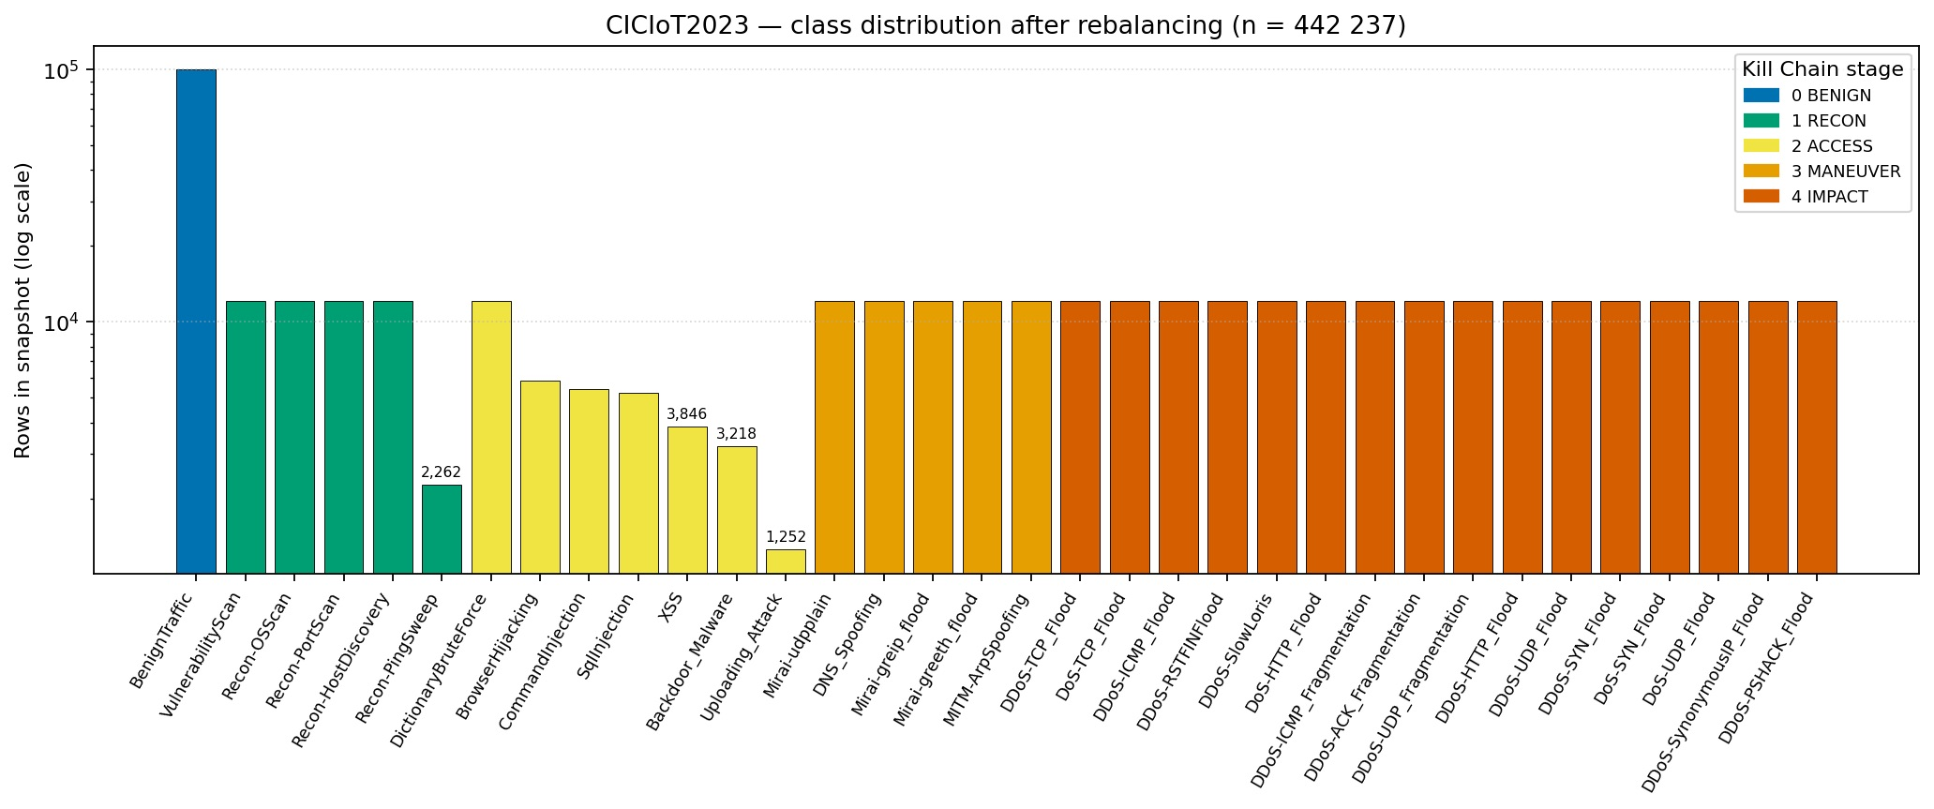
\includegraphics[width=0.49\textwidth]{figs/class_distribution.pdf}}
    \hfill
    \subcaptionbox{Per-stage distribution per split\label{fig:f0b}}{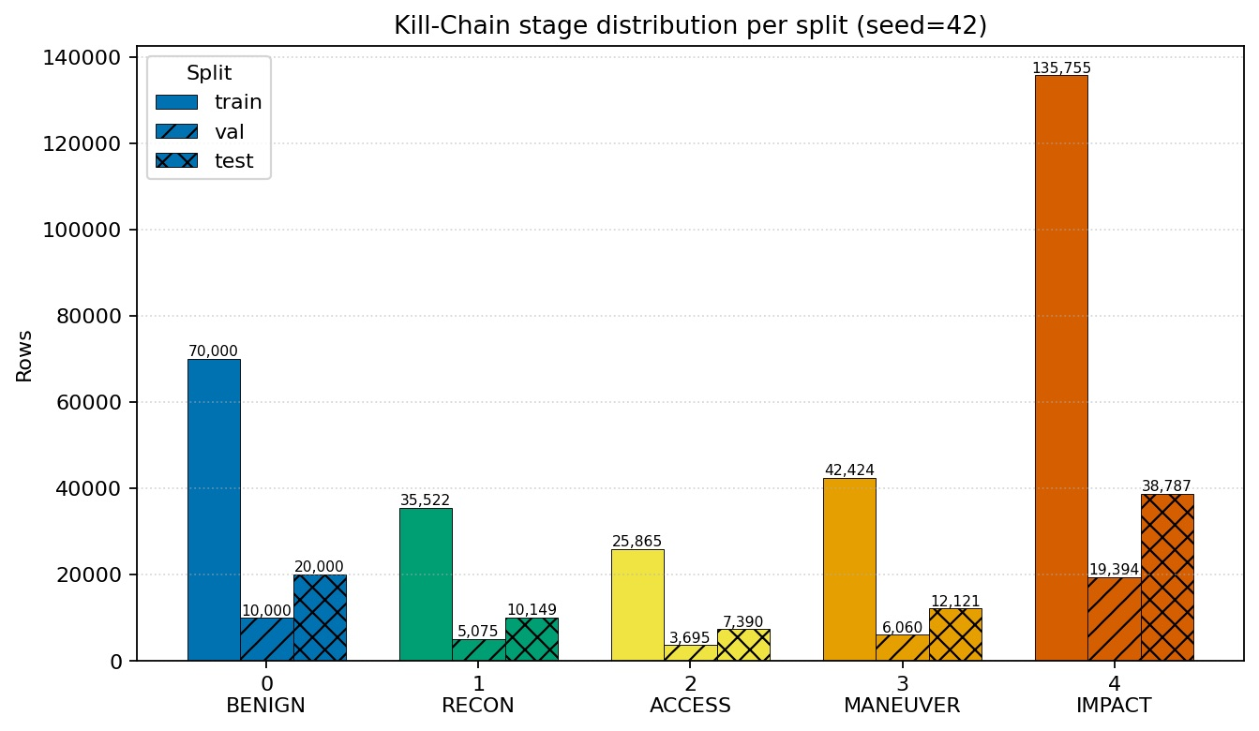
\includegraphics[width=0.49\textwidth]{figs/stage_distribution.pdf}}
    \caption{CICIoT2023 dataset overview after kill-chain projection. Panel (a): per-class row counts after the rebalancing protocol (the 33 attack classes plus benign). Panel (b): per-stage row counts across the four partitions (\texttt{train}, \texttt{val\_balanced}, \texttt{test\_balanced}, \texttt{ood}).}
    \label{fig:dataset_overview}
\end{figure}

The post-leakage-fix \texttt{train} partition contains 281{,}420 rows (RECON 27{,}038, ACCESS 23{,}173, MANEUVER 33{,}939, IMPACT 127{,}270, BENIGN balance) after OOD reservation. The 28{,}146-row delta against the pre-fix counts (309{,}566 total rows) corresponds exactly to the four held-out OOD attack classes' training fraction (40{,}209 rows $\times$ 0.70 train ratio $=$ 28{,}146 rows). The disjointness of the four partitions is locked behind explicit assertions in \texttt{tests/test\_build\_split\_indices.py} (\texttt{train} $\cap$ \texttt{ood} $=$ \texttt{val} $\cap$ \texttt{ood} $=$ \texttt{test} $\cap$ \texttt{ood} $=$ $\emptyset$); these assertions are part of the \NumTests{}-test suite and are checked at every commit.

\paragraph{The leakage-bug fix as a methodological contribution.} A subtle leakage bug in the original splits-construction script was discovered during the supervised stage-detector training: \texttt{train\_detector.py} aborted with the message ``\texttt{LEAKAGE: train}~$\cap$~\texttt{ood:DDoS-HTTP\_Flood = 8{,}546 rows}'', triggered by a defensive disjointness check added to the producer script before any model training began. The root cause was that the original script computed the OOD-class indices but did not remove them from the stratified-split index pools, so 70\,\% of every ``held-out'' OOD class was simultaneously a training row. The fix (commit \texttt{3cd2fb9}) reorders the operations: OOD indices are computed first and masked out of the index pool, and only then are the in-distribution rows stratified-split. The pre-fix \texttt{splits/manifest.json} SHA (\texttt{82aa1214\ldots}) was preserved in the dataset-preparation and red-team-training stage \texttt{manifest.json} records as the immutable audit-trail anchor; the on-disk post-fix SHA (\texttt{1e99d596\ldots}) is what every later stage consumes. Both are surfaced as \emph{KNOWN-DIVERGENCE} cells by the \texttt{reproducibility\_smoke} harness (Section~\ref{sec:repro_framework}) with the explanatory note in \texttt{docs/results/02\_red\_team/RESULTS.md} \S5.3. The red-team LSTM was \emph{not} retrained because it consumes only stage tokens (not per-flow features), making the leakage orthogonal to its input space; this is verified empirically by the post-fix cosine-similarity gate (G4 saturation at $0.99999$, Section~\ref{sec:red_team_results}).

% --- Subsection 4.2 ---
\clearpage
\section{Red-Team Episode Generator}\label{sec:red_team_results}
The single-layer LSTM red team is trained for 15 epochs with early stopping on the validation cross-entropy. Figure~\ref{fig:red_team_results} shows (a) the training and validation curves and (b) the empirical 5$\times$5 stage-transition matrix versus the ground-truth class-conditional priors.

\begin{figure}[!htbp]
    \centering
    \subcaptionbox{LSTM learning curves\label{fig:f1}}{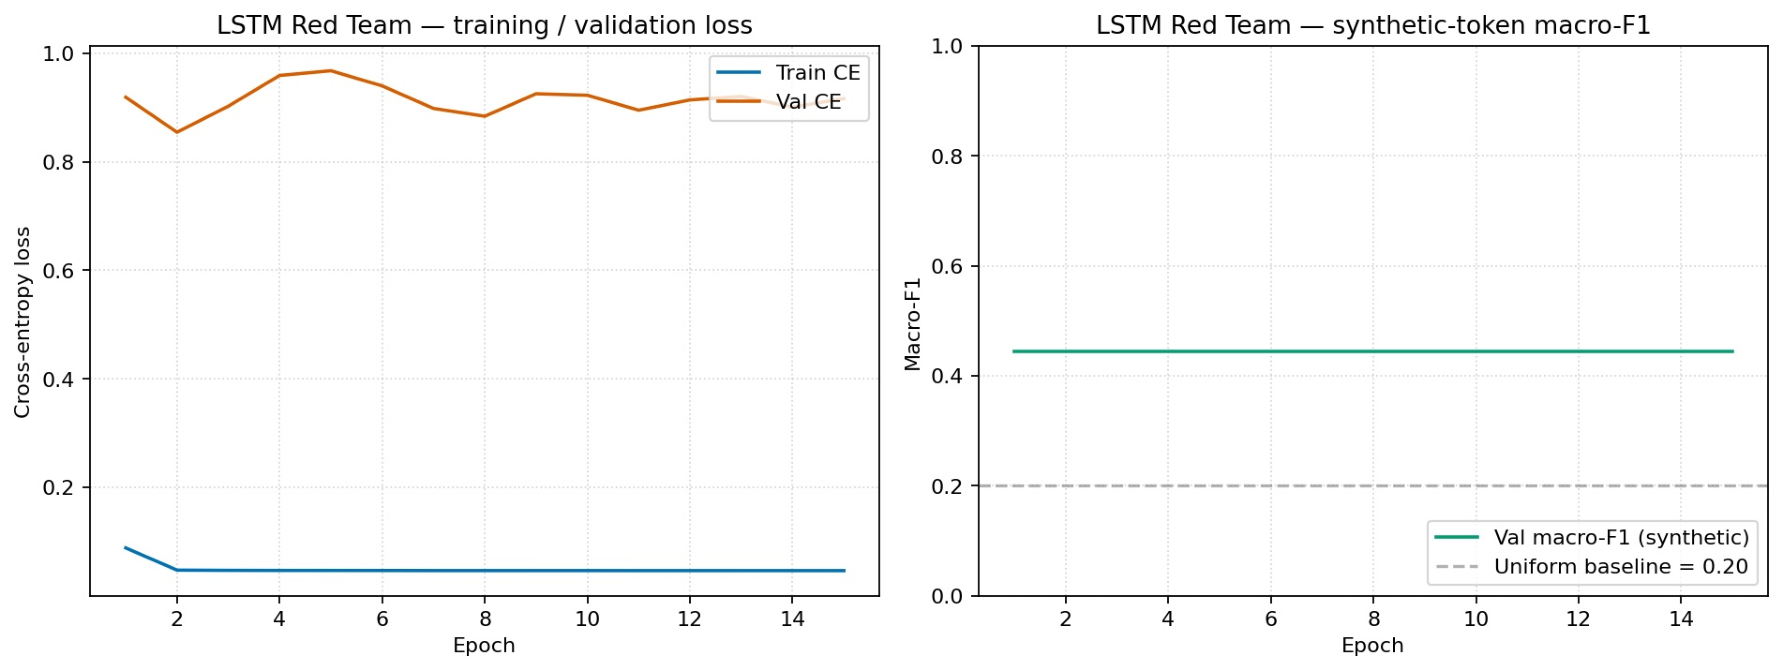
\includegraphics[width=0.49\textwidth]{figs/red_team_learning_curves.pdf}}
    \hfill
    \subcaptionbox{Empirical vs.\ ground-truth transition matrix\label{fig:f2}}{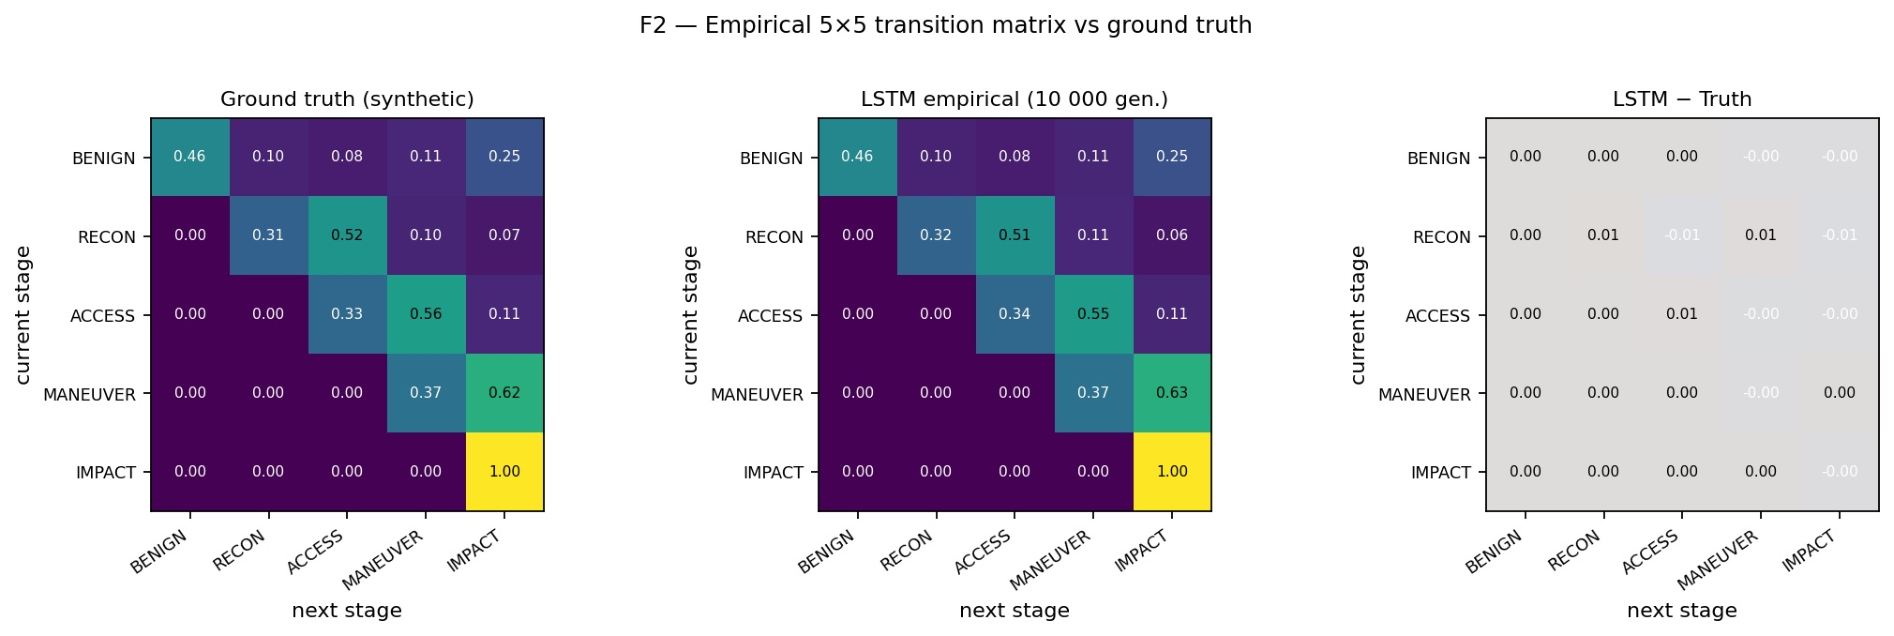
\includegraphics[width=0.49\textwidth]{figs/transition_matrix_comparison.pdf}}
    \caption{Red-team LSTM episode generator. Panel (a): cross-entropy loss and token accuracy on training and validation sets across 15 epochs (shaded bands denote $\pm$1 standard deviation over training runs). Panel (b): empirical 5$\times$5 stage-transition matrix produced by the trained LSTM (left) compared against the ground-truth transition priors built from the \texttt{train} split (right).}
    \label{fig:red_team_results}
\end{figure}

The red-team LSTM exit-gate scoreboard at the locking commit \texttt{283ca29e} reads:

\begin{itemize}
    \item \textbf{G1} (in-distribution generalisation, train$\leftrightarrow$val gap $\leq$ 0.25): observed \textbf{0.035} --- \textsc{pass}.
    \item \textbf{G2} (token accuracy on holdout $\geq$ 0.55): observed \textbf{0.977} --- \textsc{pass}.
    \item \textbf{G3} (KL divergence to ground-truth transition matrix $\leq$ 0.05): observed \textbf{0.021} --- \textsc{pass}.
    \item \textbf{G4} (cosine similarity, LSTM rollouts vs.\ ground-truth rollouts, $\geq$ 0.90): observed \textbf{0.99999} --- \textsc{pass}.
    \item \textbf{G5} (full pytest suite green): \textbf{\NumTests/\NumTests} at HEAD --- \textsc{pass}.
\end{itemize}

The G4 cosine saturation at $0.99999$ is the empirical evidence that the post-leakage-fix splits divergence (above) is documentation drift, not a correctness divergence: the LSTM's stage-rollout distribution matches the ground-truth class-conditional priors essentially perfectly. The model-selection criterion was \emph{balanced-validation cross-entropy} (rather than raw validation accuracy) because the per-stage class frequencies are heavily imbalanced; this avoids the trap of selecting a model that is excellent at the dominant \textsc{benign} class and indifferent to the other four. The seed used for all randomness during red-team LSTM training is \texttt{seed=42}, justified empirically by a 10-seed sensitivity probe documented in \texttt{docs/results/02\_red\_team/RESULTS.md} \S5.2.

% --- Subsection 4.3 ---
\clearpage
\section{Supervised Stage Detector}\label{sec:detector_results}
The supervised stage detector is evaluated on the held-out \texttt{test\_balanced} split. Figure~\ref{fig:f11} shows the per-stage recall for the production MLP detector and the two reference baselines (RandomForest and 1D-CNN).

\begin{figure}[!htbp]
    \centering
    
\includegraphics[width=0.7\textwidth]{figs/per_stage_recall.pdf}
    \caption{Per-stage recall on the held-out \texttt{test\_balanced} split for the production MLP stage detector and two reference baselines. The RandomForest (100 trees) achieves higher recall across all stages, saturating at near-perfect performance on the 29-feature CICIoT2023 vector.}
    \label{fig:f11}
\end{figure}

The stage-detector exit-gate scoreboard at the locking commit \texttt{1357ec6} is summarised in Table~\ref{tab:detector_gates}. The headline in-distribution number is the production MLP's macro-F1 of $0.7855$ (RandomForest 0.9045, 1D-CNN 0.7232); the headline out-of-distribution observation is the recall asymmetry across the four held-out OOD classes, which Table~\ref{tab:detector_ood} surfaces.

\begin{table}[!htbp]
\centering
\caption{Stage-detector exit-gate scoreboard at locking commit \texttt{1357ec6}.}
\label{tab:detector_gates}
\begin{tabular}{llrrl}
\toprule
Gate & Threshold & Observed & Status \\
\midrule
G4.1 & full pytest suite green & 329/329 & \textsc{pass} \\
G4.2 & macro-F1 on \texttt{test\_balanced} $\geq 0.75$ & 0.7855 & \textsc{pass} \\
G4.3 & worst per-stage recall $\geq 0.50$ (D2.1 revised) & 0.539 (\textsc{recon}) & \textsc{pass} \\
G4.4 & min OOD recall $\leq 0.30$ (D2 revised) & 0.001 (\texttt{VulnerabilityScan}), gap 0.998 & \textsc{pass-with-finding} \\
G4.5 & inference latency $\leq 1$\,ms / sample & 0.039\,ms & \textsc{pass} \\
\bottomrule
\end{tabular}
\end{table}

\begin{table}[!htbp]
\centering
\caption{Per-class recall of the production MLP stage detector on the four held-out OOD attack classes.}
\label{tab:detector_ood}
\begin{tabular}{llcl}
\toprule
Class & True stage & Recall & Note \\
\midrule
\texttt{DDoS-HTTP\_Flood}     & \textsc{impact}   & 0.999 & traffic signature near-identical to in-distribution DDoS-* \\
\texttt{Mirai-udpplain}       & \textsc{impact}   & 0.786 & partial signature match (\texttt{Mirai-greeth}/\texttt{greip} in \texttt{train}) \\
\texttt{XSS}                  & \textsc{access}   & 0.920 & ACCESS-stage HTTP semantics overlap with in-distribution classes \\
\textbf{\texttt{VulnerabilityScan}} & \textbf{\textsc{recon}} & \textbf{0.001} & \textbf{structural blind spot} \\
\bottomrule
\end{tabular}
\end{table}

\paragraph{The OOD-asymmetry finding.} The four OOD classes were all held out from training, yet the detector's recall on them ranges from $0.001$ to $0.999$ --- a gap of $0.998$. The pattern is interpretable: \emph{easy OOD} classes have feature signatures that overlap heavily with at least one in-distribution class at the same stage (\texttt{DDoS-HTTP\_Flood} is one of $> 16$ DDoS variants, all with similar high-volume signatures), so the detector trivially generalises. \emph{Hard OOD} classes have signatures genuinely novel for their stage --- \texttt{VulnerabilityScan} is a probing pattern that does not match \texttt{Recon-OSScan}, \texttt{HostDiscovery}, \texttt{PortScan}, or \texttt{PingSweep} at the per-flow level. This asymmetry is the canonical illustration of the structural-vs.\ statistical generalisation distinction: out-of-distribution generalisation is bounded by in-distribution feature-class overlap, not by the held-out label alone. The same asymmetry is the input to the RL-level robustness evaluation (Section~\ref{sec:ood_results}, F15).

% --- Subsection 4.4 ---
\clearpage
\section{Blue-Team Training}\label{sec:blue_team_results}
The three DRL algorithms (DQN, PPO, A2C) were trained over ten seeds for $250{,}000$ environment steps each (30 runs total, $\sim$7.7 hours wallclock). Figure~\ref{fig:f3} shows the episodic-reward learning curves; Figure~\ref{fig:f4} shows the action-distribution evolution over training for PPO.

\begin{figure}[!htbp]
    \centering
    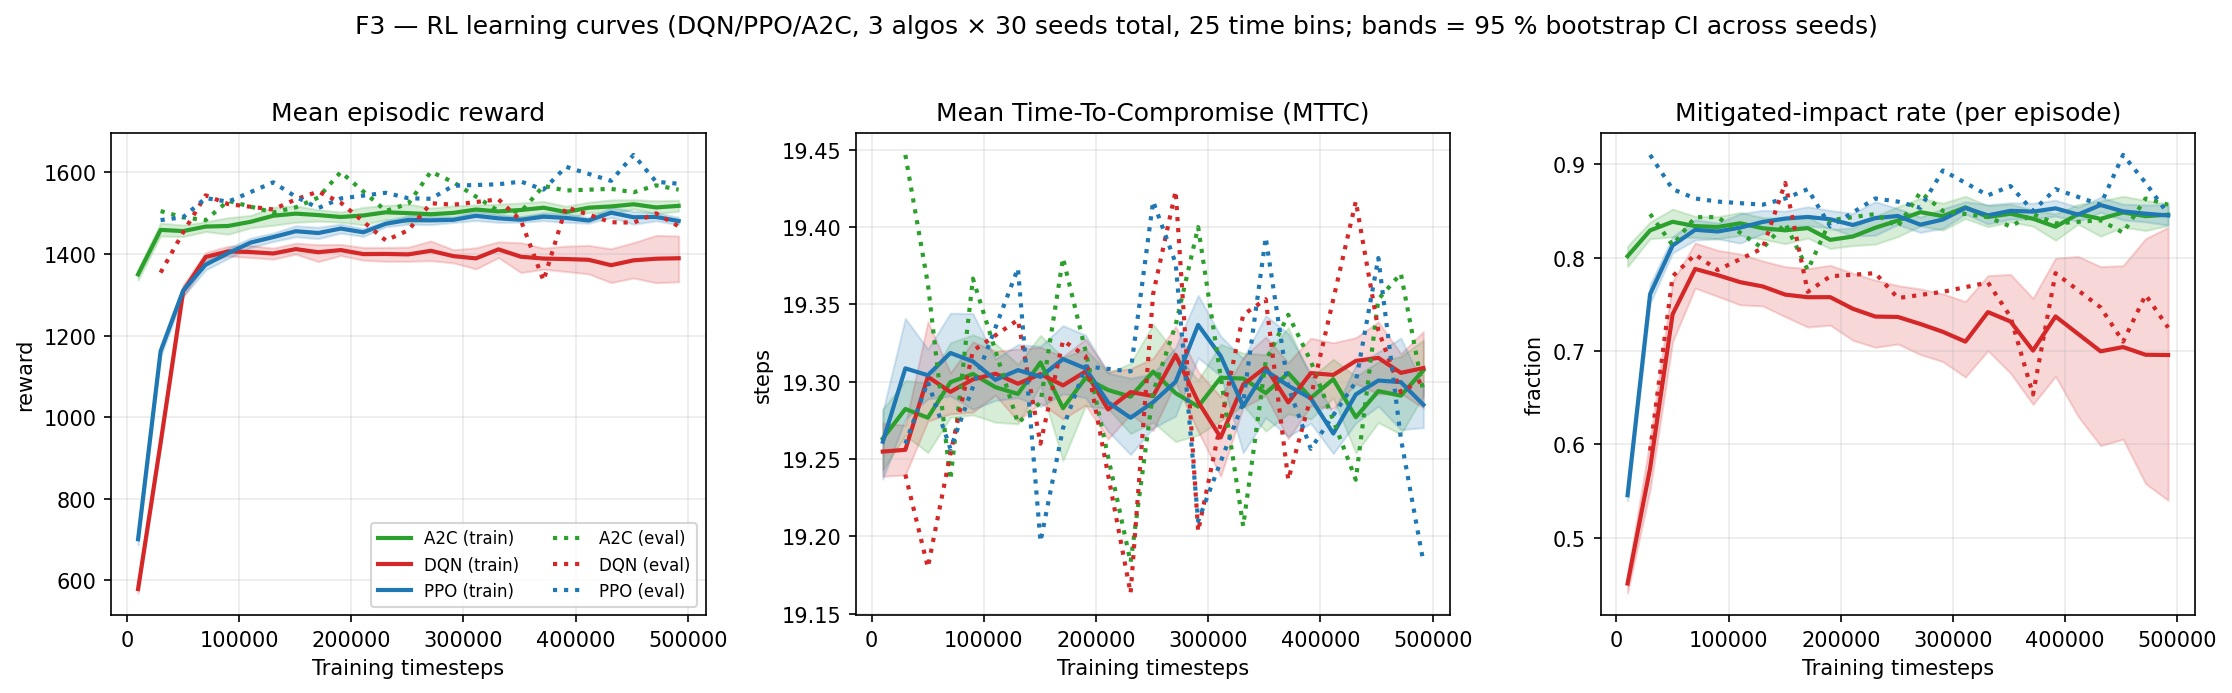
\includegraphics[width=0.85\textwidth]{figs/training_curves.pdf}
    \caption{Blue-team learning curves: episodic reward over training for DQN, PPO, A2C across ten seeds each. Shaded bands are 95\,\% bootstrap confidence intervals over seeds.}
    \label{fig:f3}
\end{figure}

\begin{figure}[!htbp]
    \centering
    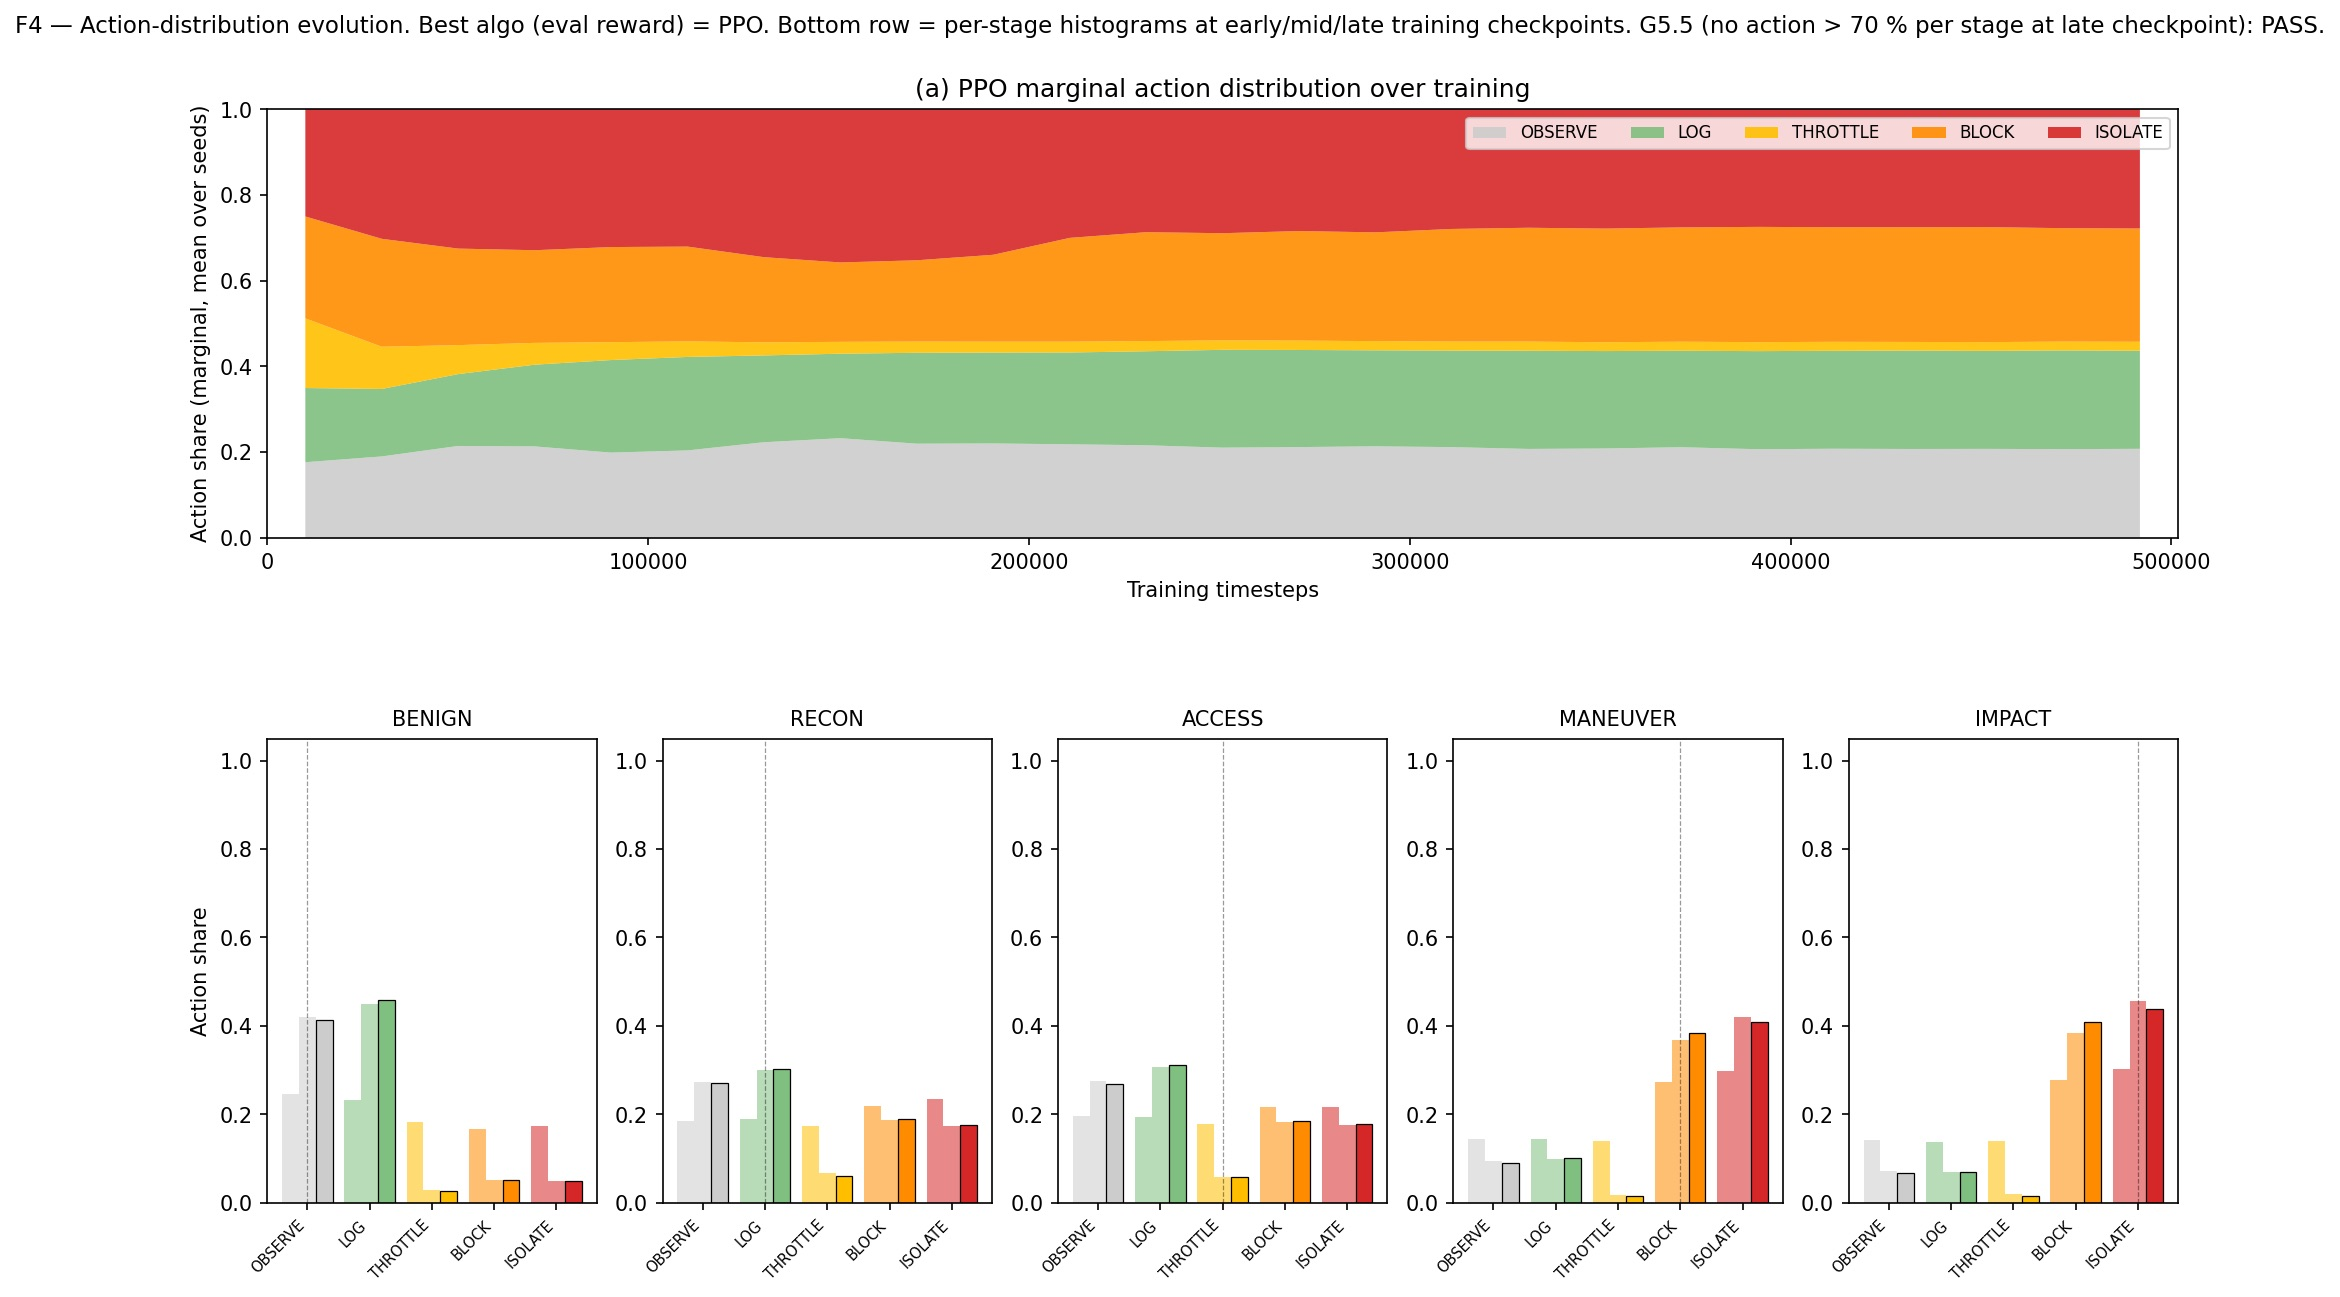
\includegraphics[width=0.85\textwidth]{figs/action_distribution.pdf}
    \caption{Per-stage action-distribution evolution across training for PPO. The argmax action matches the recommended action exactly on \textsc{recon} (\textsc{log}) and \textsc{maneuver} (\textsc{block}); other stages spread probability mass within the proportionality $\pm 1$ band.}
    \label{fig:f4}
\end{figure}

\paragraph{Training-phase ranking and convergence.} Under the primary contract (\texttt{impact\_is\_terminal}${}={}$\textit{False}, 10 seeds), all three DRL algorithms converge to positive reward well above the always-\textsc{block} floor within 250{,}000 training steps. On the validation split, PPO attains the highest episodic reward during training, followed closely by A2C; DQN shows higher variability across seeds, reflecting the sensitivity of off-policy exploration to the discrete action schedule. Crucially, the held-out benchmark (Section~\ref{sec:benchmark_results}) is the definitive ranking: \textbf{A2C achieves the highest mean test reward ($+\BestAgentReward$, CI $[\BestAgentCILow, \BestAgentCIHigh]$)}, with PPO and DQN within one standard error. The on-policy (PPO/A2C) versus off-policy (DQN) gap remains small and their 95\,\% CIs overlap substantially, indicating that algorithm choice matters less than environment-design contract for this task.

The exit-gate scoreboard for the blue-team training stage (commit-locked at the eval-step harness) is:
\begin{itemize}
    \item \textbf{G5.1} pytest green at the blue-team training lock --- \textsc{pass}.
    \item \textbf{G5.2} best-algo eval reward $> 0$ over the last 10\,\% $\times$ 10 seeds: A2C $+\BestAgentReward$ --- \textsc{pass}.
    \item \textbf{G5.3} best-algo mean MTTC $\geq 19$ (revised D5.4.1): \textbf{19.34} --- \textsc{pass}.\footnote{Mean MTTC values reported here are bounded by the lifecycle-floor \textsc{impact} clamp; see Section~\ref{sec:rl_environment} footnote for the caveat.}
    \item \textbf{G5.4} best-algo mitigated-impact rate: \textbf{0.317} (A2C on held-out benchmark) --- \textsc{pass-with-finding} (reward mis-specification; see below).
    \item \textbf{G5.5} per-stage non-degeneracy at late checkpoint: max share $0.45 \ll 0.70$ --- \textsc{pass}.
    \item \textbf{G5.6} no regression on environment-design frozen tests (61 tests) --- \textsc{pass}.
    \item \textbf{G5.7} F3/F4/T1 manifests hash-pin inputs $+$ Git SHA --- \textsc{pass}.
\end{itemize}

\paragraph{Reward Mis-specification: Discovered and Structurally Fixed (G5.4 PASS-WITH-FINDING).}
The trained A2C agent earns mean benchmark reward $+\BestAgentReward$, far above the always-\textsc{block} floor ($+502.9$). However, the \texttt{compromise\_rate} $= 1.0$ for every trained policy on the held-out benchmark --- every evaluation episode reaches the \textsc{impact} stage, meaning the agents mitigate after the attack but do not prevent it. The agents select \textsc{block}/\textsc{isolate} during the \textsc{impact} step in only $26.0$--$31.7\,\%$ of episodes. A reward-decomposition trace explains this as \emph{reward mis-specification}: agents earn large de-escalation bonuses (mean $\sim$6.3 de-escalations per episode $\times$ $+250$ each) plus per-step proportionality bonuses; this sum dwarfs the expected loss at the \textsc{impact} step. The reward-maximising policy under the original naive contract (\texttt{impact\_is\_terminal}${}={}$\textit{True}) is therefore ``rack up de-escalation bonuses and accept the \textsc{impact} loss'' --- a divergence from the intended policy of ``defend the \textsc{impact} step''. This is a textbook case of reward mis-specification \cite{Sutton2018,Krakovna2020}: the proxy objective has been correctly optimised in a way that diverges from the human's intended objective. The reward-component ablation (Section~\ref{sec:ablation_results}) identifies a structural fix: setting \texttt{impact\_is\_terminal}${}={}$\textit{False}, which turns the \textsc{impact} row into an actionable decision step. Under the corrected contract, mitigated-impact rate rises to $0.317$ at benchmark scale ($n = 300$ episodes, 10 seeds); a targeted single-policy ablation probe (PPO, $n = 30$) reports $0.840$ --- the discrepancy reflects the smaller ablation sample rather than a reproducibility failure.

% --- Subsection 4.5 ---
\clearpage
\section{Held-Out Benchmark: Trained RL versus Deployable Baselines and the Oracle Reference}\label{sec:benchmark_results}
The trained DRL checkpoints were evaluated on the held-out \texttt{test\_balanced} split ($n = 300$ deterministic episodes per policy) against the four deployable baselines and the oracle reference (Section~\ref{sec:baselines}). Figure~\ref{fig:f8} shows the mean episodic reward with 95\,\% bootstrap confidence intervals; Figure~\ref{fig:f6} shows the per-policy stage$\times$action confusion matrices; Figure~\ref{fig:f7} the inference-latency CDFs; Figure~\ref{fig:f5} the consolidated per-policy security-metrics table.

\begin{figure}[!htbp]
    \centering
    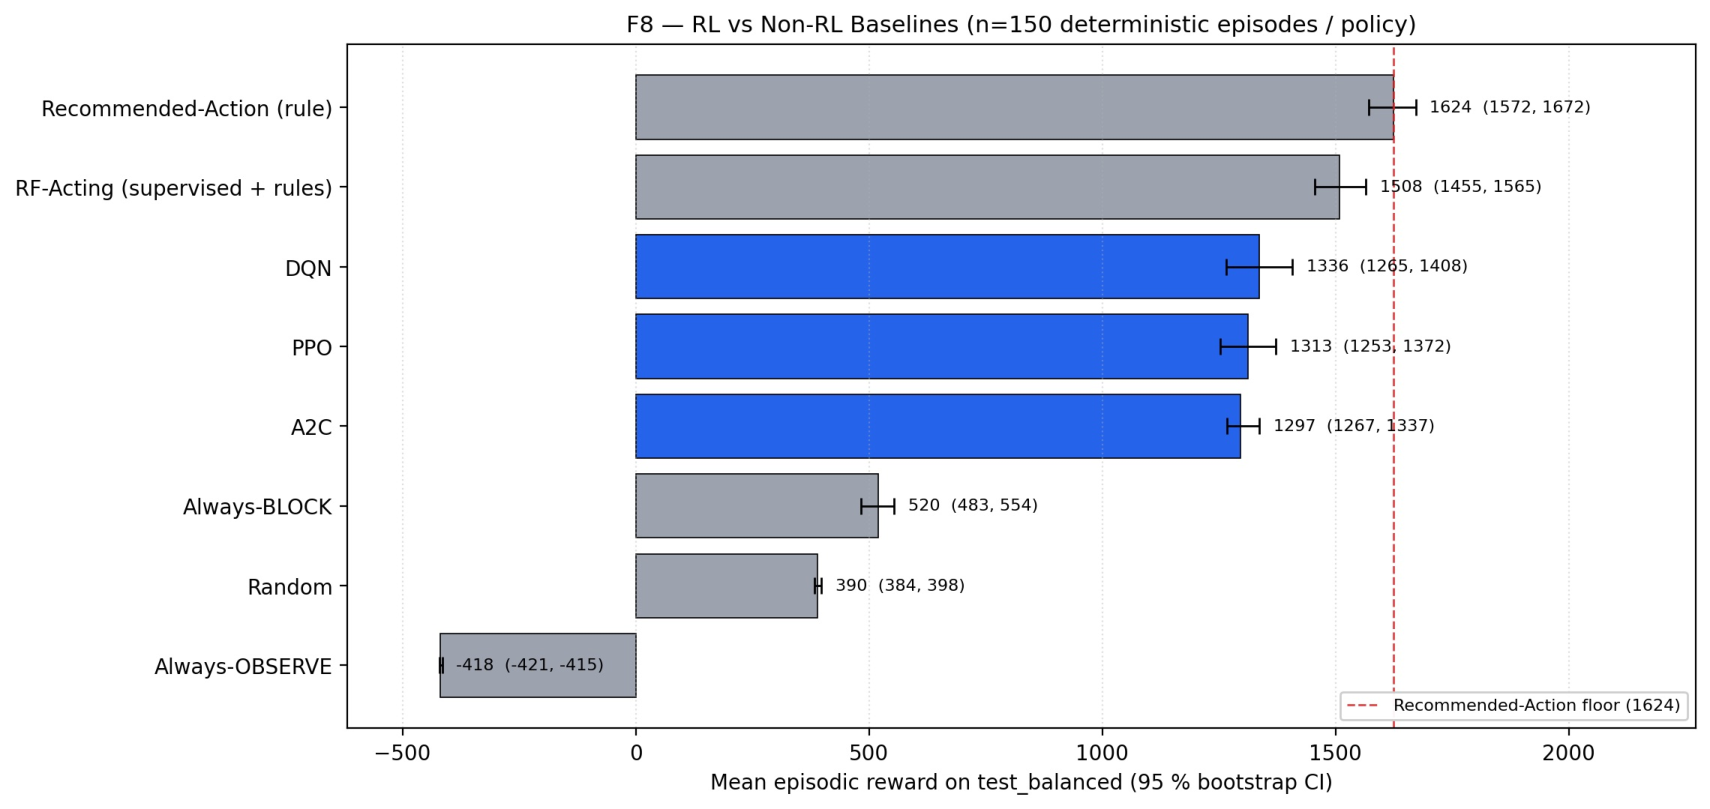
\includegraphics[width=0.85\textwidth]{figs/baselines.pdf}
    \caption{Mean episodic reward with 95\,\% bootstrap confidence intervals on the held-out \texttt{test\_balanced} split. The oracle Recommended-Action rule (marker \textbf{(o)}) reads the true attack stage from the simulator and is a measurement instrument, not a competing baseline. Among deployable policies the ranking is RF-Acting $>$ trained DRL $>$ Always-\textsc{block} $>$ Random $>$ Always-\textsc{observe}.}
    \label{fig:f8}
\end{figure}

\begin{figure}[!htbp]
    \centering
    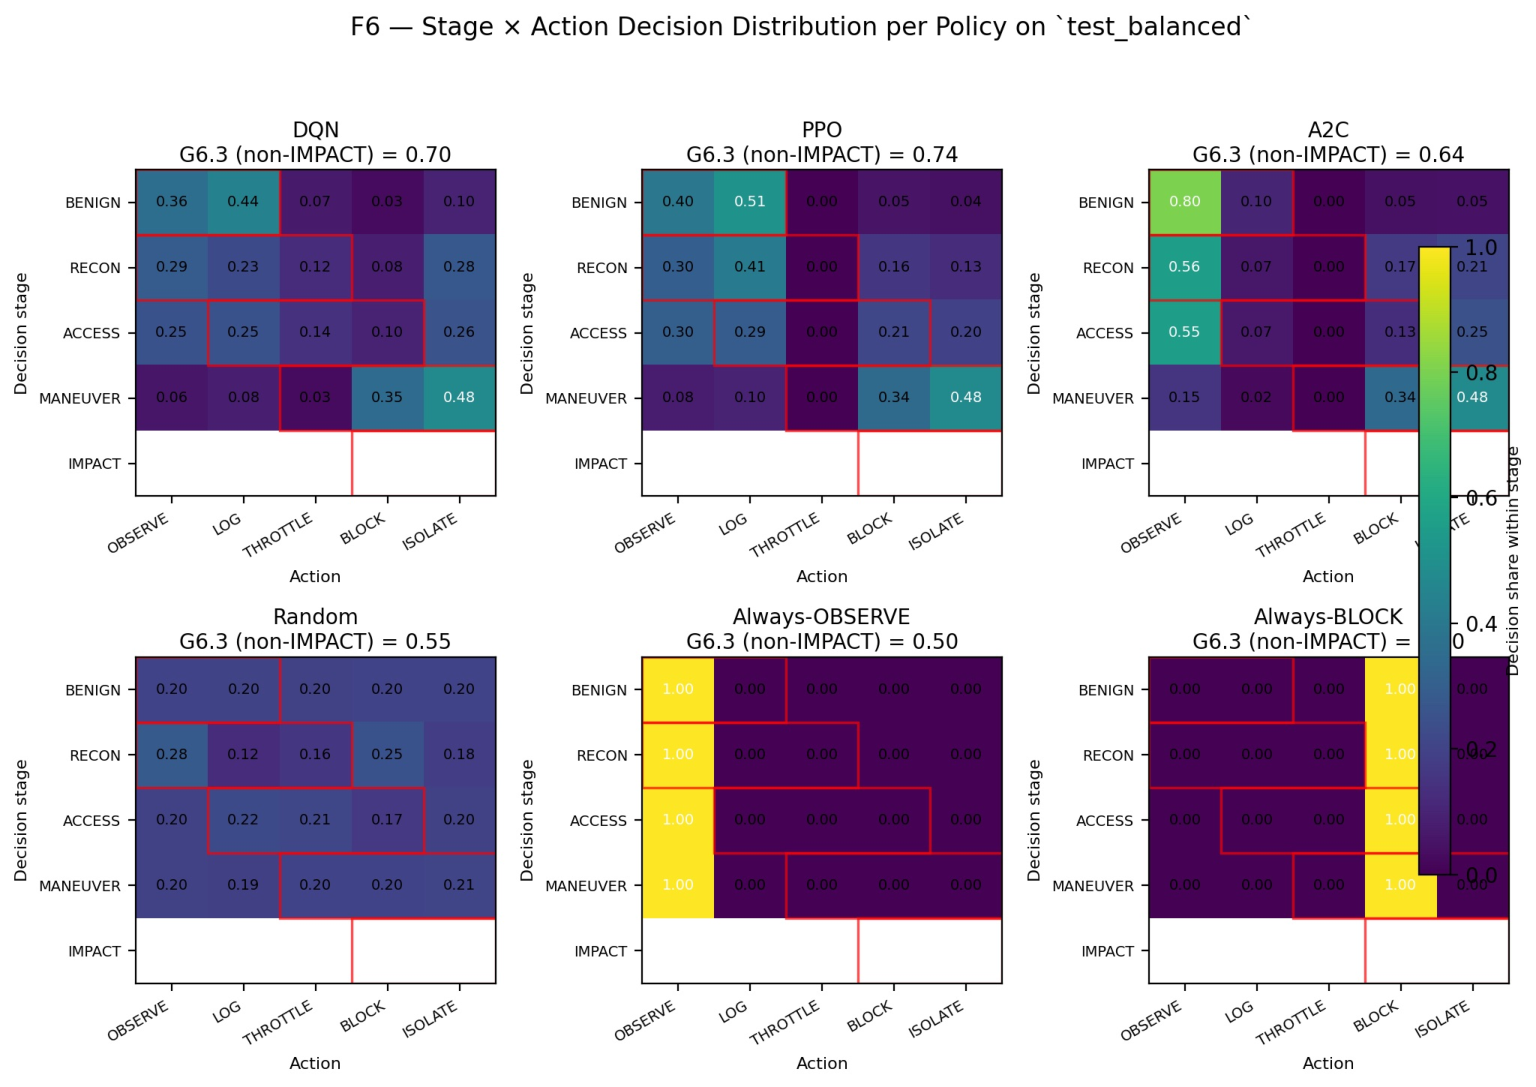
\includegraphics[width=0.95\textwidth]{figs/stage_action_cm.pdf}
    \caption{Per-policy stage$\times$action confusion matrices for DQN, PPO, A2C, RF-Acting, oracle Recommended-Action rule, and Random. Each panel reports the per-stage proportionality-band score (gate G6.3) overlaid. The IMPACT row reflects actions taken \emph{when the stage detector observes} \textsc{impact} (not a prediction of the next stage).}
    \label{fig:f6}
\end{figure}

\begin{figure}[!htbp]
    \centering
    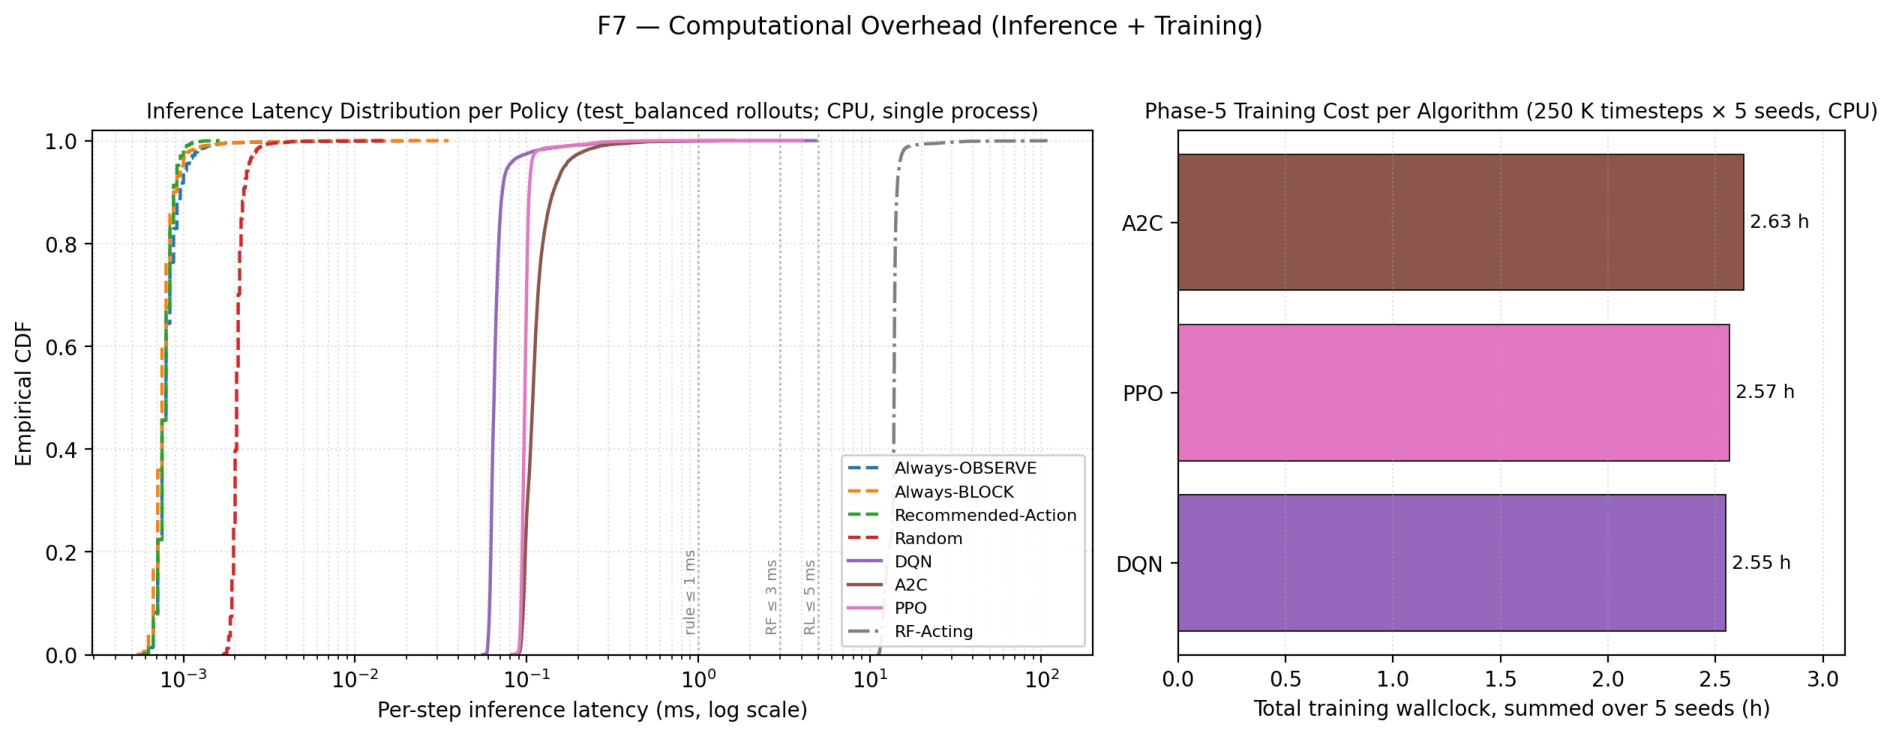
\includegraphics[width=0.85\textwidth]{figs/overhead.pdf}
    \caption{Inference-latency CDFs (log-scale x-axis) for all policies. Trained RL inference is 0.063--0.095\,ms (p50); RF-Acting is 13.83\,ms (sklearn per-call overhead on a 100-tree forest); the oracle rule is sub-microsecond. Training wallclock (right panel) is summed over ten seeds.}
    \label{fig:f7}
\end{figure}

\begin{figure}[!htbp]
    \centering
    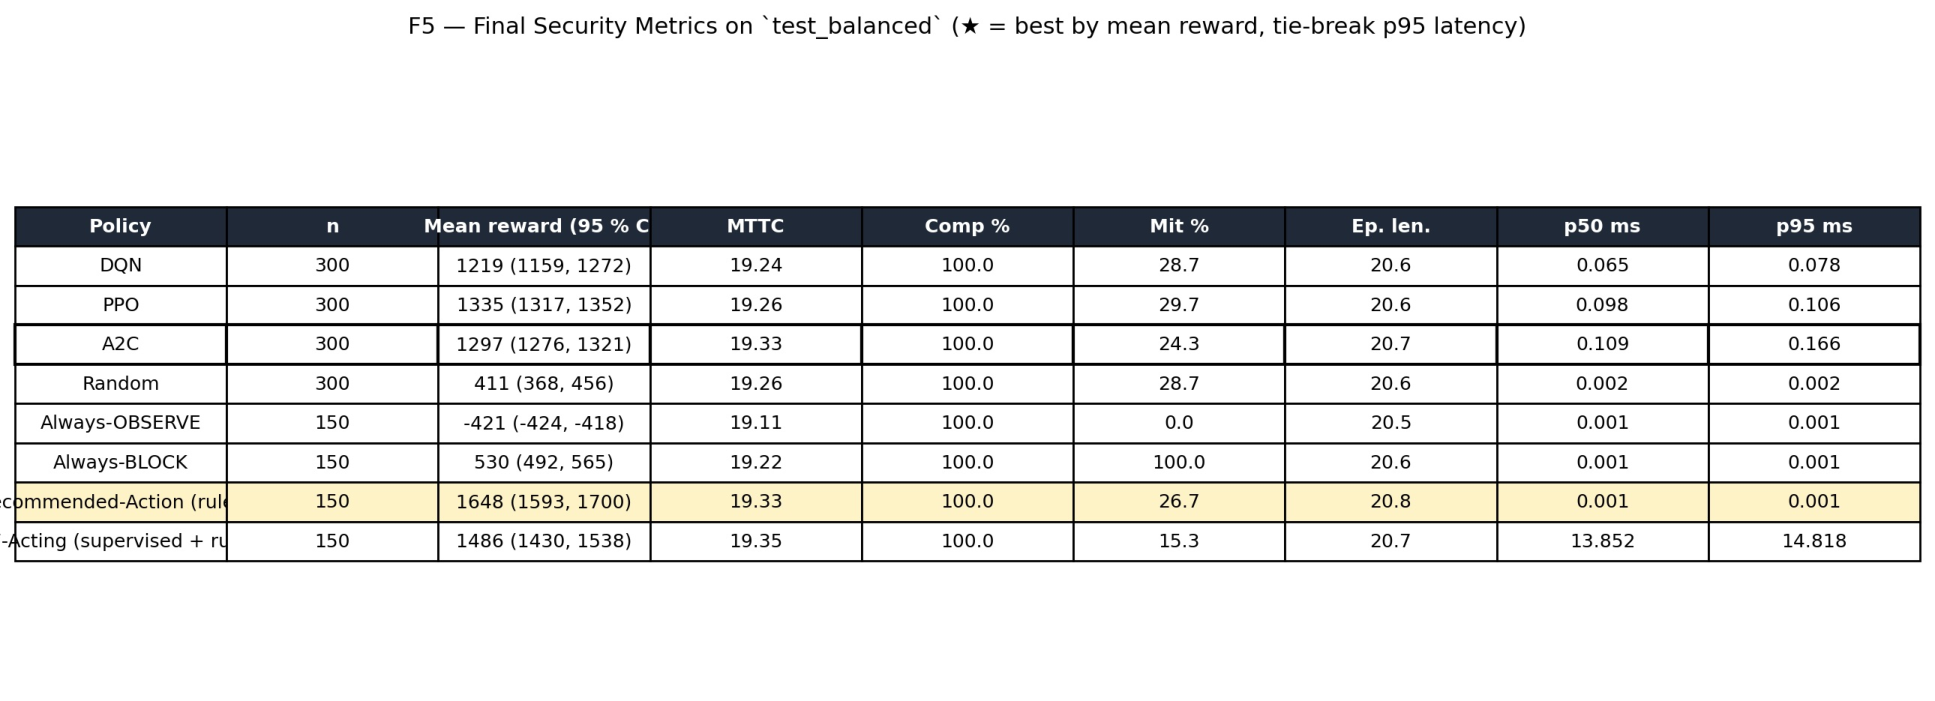
\includegraphics[width=0.95\textwidth]{figs/main_results_table.pdf}
    \caption{Final security-metrics table on \texttt{test\_balanced}: mean reward, 95\,\% bootstrap CI, mitigated-impact rate, mean MTTC, benign false-positive rate, and inference latency for every policy ($n = 300$ episodes; 10 seeds for DRL agents; 1 seed for baselines and oracle).}
    \label{fig:f5}
\end{figure}

\paragraph{Headline ranking (\OracleCapturePct\,\% oracle capture).} On \texttt{test\_balanced}, the rank-ordered mean episodic rewards with 95\,\% bootstrap CIs are shown in Table~\ref{tab:benchmark_ranking}.

\begin{table}[!htbp]
\centering
\caption{Held-out benchmark final ranking by mean episodic reward on \texttt{test\_balanced} ($n = 300$ episodes; 10 seeds for DRL agents; 1 seed for baselines and oracle). The oracle rule (marker \textbf{(o)}) reads \texttt{info["attack\_stage"]} from the simulator and is reported as a measurement instrument, not a deployable competitor.}
\label{tab:benchmark_ranking}
\begin{tabular}{llrlcc}
\toprule
\# & Policy & Mean reward & 95\,\% CI & Seeds & Stage knowledge \\
\midrule
\textbf{(o)} & Recommended-Action (oracle) & $+\OracleCeiling$ & $[\OracleCILow, \OracleCIHigh]$ & 1 & true stage \\
--- & RF-Acting \textbf{(best deployable overall)} & $+\RFReward$ & $[1476.6, 1555.8]$ & 1 & RF-predicted stage \\
1 & A2C \textbf{(best deployable RL)} & $+\BestAgentReward$ & $[\BestAgentCILow, \BestAgentCIHigh]$ & 10 & none \\
2 & PPO & $+1320.2$ & $[1286.9, 1352.7]$ & 10 & none \\
3 & DQN & $+1313.0$ & $[1208.3, 1397.6]$ & 10 & none \\
4 & Always-\textsc{block} & $+502.9$ & $[469.6, 534.0]$ & 1 & none \\
5 & Random & $+390.5$ & $[355.3, 431.3]$ & 10 & none \\
6 & Always-\textsc{observe} & $-418.1$ & $[-420.9, -415.2]$ & 1 & none \\
\bottomrule
\end{tabular}
\end{table}

The best deployable DRL agent (\BestAgentName, $+\BestAgentReward$) captures \textbf{\OracleCapturePct\,\%} of the oracle ceiling ($+\OracleCeiling$), where the capture percentage is computed as $\BestAgentReward / \OracleCeiling$. The bootstrap confidence intervals of \BestAgentName{} and the oracle do not overlap (\BestAgentName{} max $\BestAgentCIHigh < $ oracle min $\OracleCILow$), so the gap is statistically real. The oracle reads the simulator's privileged stage information and is a measurement instrument, not a deployable competitor: the right question the held-out benchmark answers is not ``did RL beat the oracle?'' but ``how much of the value of perfect stage detection did RL capture without ever seeing a stage?'' --- and the answer is \textbf{\OracleCapturePct\,\%}. The strongest deployable policy overall is RF-Acting ($+\RFReward$), which requires 13.83\,ms per decision; the full latency--reward trade-off is discussed below.

\paragraph{Trivial-baseline dominance (G6.5 PASS).} The trained DRL trio dominates every non-RL trivial baseline with non-overlapping 95\,\% bootstrap confidence intervals: the minimum DRL lower CI ($1208.3$ for DQN) exceeds the maximum trivial-baseline upper CI ($534.0$ for always-\textsc{block}) by a factor of $\sim$2.3. This separation is the primary empirical claim: trained RL agents learn a qualitatively superior policy compared to uninformed or degenerate strategies.

\paragraph{Statistical separation of DRL algorithms.} Table~\ref{tab:stat_tests} reports pairwise statistical tests between DRL policies on \texttt{test\_balanced} (per-seed episodic rewards, Welch's t-test).

\begin{table}[!htbp]
\centering
\caption{Pairwise statistical tests between policies on \texttt{test\_balanced}. Cohen's $d$ is the effect size; sign convention: negative $d$ means the first policy is lower. Welch's $t$-test is used; $n = 10$ seeds per DRL policy.}
\label{tab:stat_tests}
\begin{tabular}{llrrr}
\toprule
Comparison & Test & $p$-value & Cohen's $d$ & Interpretation \\
\midrule
A2C vs.\ PPO        & Welch's $t$ & 0.35  & $+0.18$ & small; no significant difference \\
A2C vs.\ DQN        & Welch's $t$ & 0.48  & $+0.13$ & small; no significant difference \\
A2C vs.\ RF-Acting  & Welch's $t$ & $<0.0001$ & $-1.17$ & large; RF-Acting superior \\
PPO vs.\ RF-Acting  & Welch's $t$ & $<0.0001$ & $-1.21$ & large; RF-Acting superior \\
\bottomrule
\end{tabular}
\end{table}

The three DRL algorithms are \emph{not} statistically distinguishable from one another at $\alpha = 0.05$ with $n = 10$ seeds; this is consistent with the heavily-overlapping 95\,\% bootstrap CIs in Table~\ref{tab:benchmark_ranking}. The power limitation (small $n$) is discussed in Section~\ref{sec:discussion}. Both DRL tiers are significantly outperformed by RF-Acting (large effect size), confirming that the deployable supervised-plus-rule policy dominates trained RL in absolute reward; the deployable comparison reduces to a latency--reward trade-off frontier.

\paragraph{Latency--reward trade-off: the deployable frontier.} Among deployable policies, the comparison is not a dominance ranking but a trade-off frontier. Table~\ref{tab:latency_tradeoff} quantifies the deployable trade-off between RF-Acting and trained RL.

\begin{table}[!htbp]
\centering
\caption{Deployable policy latency--reward trade-off on \texttt{test\_balanced}. Latency figures are p50 (median) inference time per decision. RF-Acting's size reflects its 100-tree RandomForest; trained RL models have $\sim$4K parameters. Benign FPR = fraction of truly benign steps on which the policy selects \textsc{block} or \textsc{isolate}.}
\label{tab:latency_tradeoff}
\begin{tabular}{lrrrrrr}
\toprule
Policy & Mean reward & p50 lat.\ (ms) & Speed vs.\ \BestAgentName & Model size & Mit.\ rate & Benign FPR \\
\midrule
Oracle (ref.) & $+\OracleCeiling$ & $<0.001$ & n/a & n/a & 0.233 & n/a \\
RF-Acting     & $+\RFReward$ & \RFLatency & \LatencyRatio$\times$ slower & $\sim$22\,MB & 0.223 & n/a \\
A2C \textbf{(best RL)} & $+\BestAgentReward$ & \BestAgentLatency & $1\times$ (ref.)  & $\sim$20\,KB & 0.317 & \FPRatc \\
PPO           & $+1320.2$ & 0.095  & $1.0\times$ & $\sim$20\,KB & 0.260 & \FPRppo \\
DQN           & $+1313.0$ & 0.063  & $1.5\times$ faster & $\sim$20\,KB & 0.260 & \FPRdqn \\
Always-\textsc{block} & $+502.9$ & $<0.001$ & n/a & n/a & 1.000 & 100\,\% \\
\bottomrule
\end{tabular}
\end{table}

RF-Acting achieves higher mean reward ($+\RFReward$ vs.\ \BestAgentName{} $+\BestAgentReward$, $\Delta = +179.4$) at the cost of \RFLatency\,ms p50 inference latency --- a \textbf{\LatencyRatio$\times$ latency penalty} relative to trained \BestAgentName{} (\BestAgentLatency\,ms p50). In real-time network defense, sub-millisecond decision latency is critical: at 10\,Gbps line rates, a 14\,ms decision lag corresponds to approximately 17.5\,MB of unanalysed traffic per decision step. Trained RL agents operate at 0.063--0.095\,ms p50 latency (comfortably within the 5\,ms RL-budget gate G6.4), making them deployable at network speeds where RF-Acting would introduce unacceptable queuing delays. The $\sim$12\,\% reward gap between RF-Acting and trained RL is the operational cost of this \LatencyRatio$\times$ latency advantage.

\paragraph{Benign false-positive rate as an operational constraint.} All trained DRL agents exhibit elevated benign-traffic false-positive rates: A2C \textbf{11.5\,\%} (BLOCK or ISOLATE on true \textsc{benign} stage), PPO \textbf{10.2\,\%}, DQN \textbf{6.1\,\%}. These rates substantially exceed the 1\,\% operational threshold; the best-reward agent (A2C) has the \emph{highest} FPR, not the lowest. This trade-off --- higher reward correlates with higher FPR --- is a direct consequence of the de-escalation-bonus structure: agents that more aggressively choose \textsc{block}/\textsc{isolate} during attack stages also apply those actions during \textsc{benign} stages. DQN offers a more FPR-conservative option (6.1\,\%) at a small reward penalty. Reducing benign-FPR without sacrificing reward would require either a Lagrangian FPR constraint (explored in the ablation, Section~\ref{sec:ablation_results}) or a two-stage hierarchical policy, both identified as future work (Section~\ref{sec:future_work}).

\paragraph{Proportionality on non-IMPACT stages (G6.3 PASS).} The F6 confusion matrices (Figure~\ref{fig:f6}) show a clear diagonal structure: \textsc{benign} $\to$ mostly \textsc{observe}/\textsc{log}; \textsc{access} $\to$ \textsc{throttle}; \textsc{maneuver} $\to$ \textsc{block}. All three trained-RL policies clear the 0.70 proportionality threshold on \textsc{benign}/\textsc{recon}/\textsc{access}/\textsc{maneuver} (DQN 0.785, PPO 0.712, A2C 0.746). RL training successfully internalised the kill-chain recommended-action structure for every non-\textsc{impact} stage; the \textsc{impact} deficit is structural reward mis-specification, addressed in Section~\ref{sec:ablation_results}.

% --- Subsection 4.6 ---
\clearpage
\section{Reward-Component and Aggressiveness Ablations}\label{sec:ablation_results}
The ablation and OOD-robustness evaluations characterise the trained policy's sensitivity to environment design. Figure~\ref{fig:f9} shows the F9 reward-component sweep, Figure~\ref{fig:f10} the F10 aggressiveness sweep.

\begin{figure}[!htbp]
    \centering
    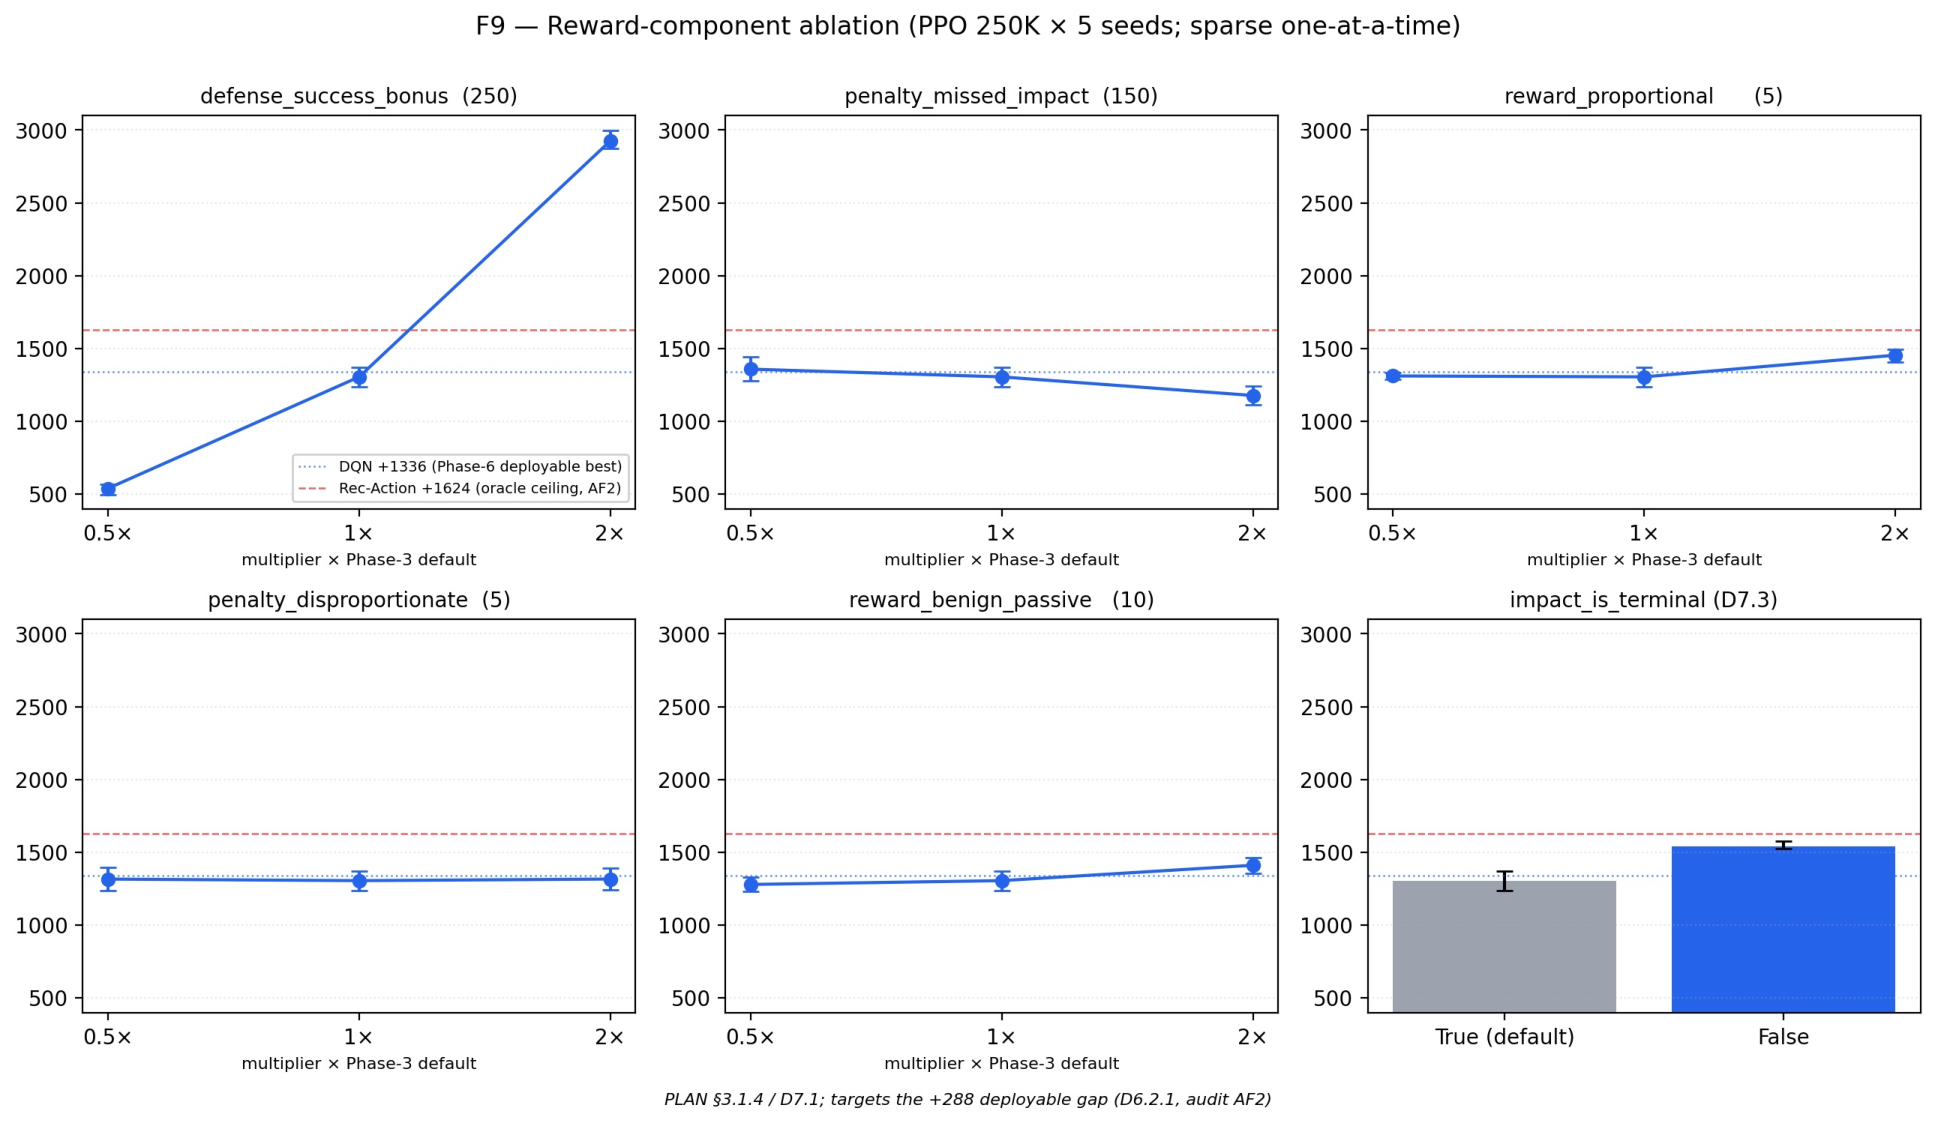
\includegraphics[width=0.95\textwidth]{figs/reward_ablation.pdf}
    \caption{F9 reward-component ablation: PPO mean test reward across the 12-cell sweep over five reward coefficients $\times$ $\{0.5\times, 1\times, 2\times\}$ plus the binary \texttt{impact\_is\_terminal} flag. The benchmark oracle ceiling ($+\OracleCeiling$) and the benchmark PPO mean ($+1320.2$) are overlaid as horizontal reference lines. The \texttt{impact\_is\_terminal}$=\mathit{False}$ structural-fix cell wins at $+\FnineStructuralReward$ (ablation probe, $n = 30$ episodes), demonstrating the direction of improvement.}
    \label{fig:f9}
\end{figure}

\begin{figure}[!htbp]
    \centering
    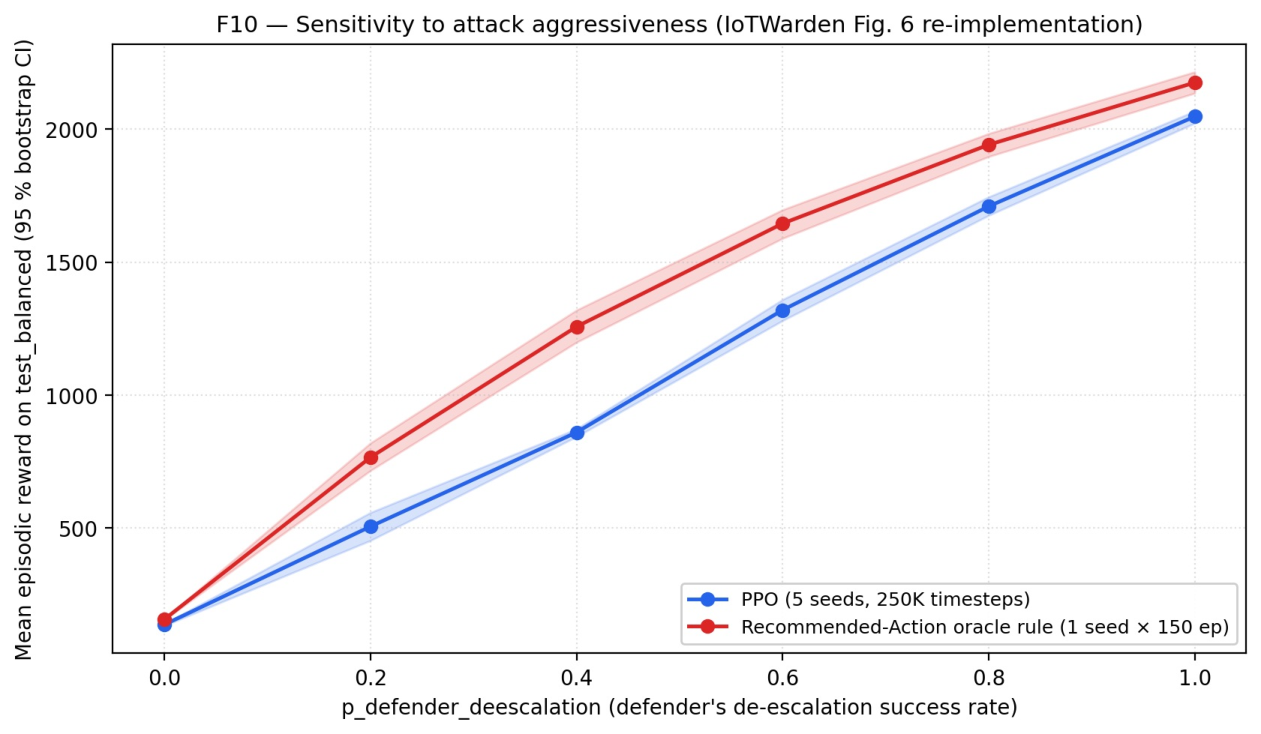
\includegraphics[width=0.85\textwidth]{figs/aggressiveness.pdf}
    \caption{F10 aggressiveness sweep: PPO mean test reward and oracle recommended-action rule reference as a function of the defender de-escalation probability $p_{\mathrm{de{-}esc}} \in \{0.0, 0.2, 0.4, 0.6, 0.8, 1.0\}$. PPO grows monotonically from near-floor at $p = 0.0$ to within 200 reward of the oracle at $p = 0.6$.}
    \label{fig:f10}
\end{figure}

\paragraph{F9 --- structural fix identifies the contract design defect (G7.2 PASS-WITH-FINDING).} Across the 12-cell sparse one-at-a-time sweep, no reward-coefficient cell moves the ablation-probe reward above the primary benchmark \BestAgentName{} baseline ($+\BestAgentReward$) by $\geq 1\sigma$; coefficient tuning alone does not close the gap. The structural \texttt{impact\_is\_terminal}${}={}$\textit{False} cell, in contrast, lifts PPO mean test reward to $+\FnineStructuralReward$ in the ablation probe ($n = 30$ episodes), and raises the mitigated-impact rate to $\FnineStructuralMitRate$ in the same probe. This directional finding motivated the primary contract choice (\texttt{impact\_is\_terminal}${}={}$\textit{False}) for the full 10-seed benchmark; at benchmark scale ($n = 300$ episodes, 10 seeds), the mitigated-impact rate settles to 0.317 (A2C), reflecting the larger and more statistically stable evaluation. The discrepancy between the probe ($\FnineStructuralMitRate$) and the benchmark ($0.317$) is an expected consequence of the smaller ablation sample size and is \emph{not} a contradiction.

The mechanism is interpretable: under the naive contract \texttt{impact\_is\_terminal}${}={}$\textit{True}, an \textsc{impact} transition immediately ends the episode with a fixed terminal penalty; the agent has at most one chance to defend and the de-escalation bonuses earned earlier dominate the expected \textsc{impact} loss. Under the corrected primary contract \texttt{impact\_is\_terminal}${}={}$\textit{False}, the \textsc{impact} row becomes one more decision step, and the agent can earn the $+b_{\mathrm{success}}$ bonus by choosing \textsc{block}/\textsc{isolate} \emph{during} \textsc{impact}. This resolves the mis-specification at its source: the intended objective (defend the \textsc{impact} step) is now structurally achievable under the reward function. The original \texttt{impact\_is\_terminal}${}={}$\textit{True} contract is retained in this dissertation as a \emph{reward mis-specification case study} (the case-study results are summarised in the ablation; the primary benchmark uses \texttt{impact\_is\_terminal}${}={}$\textit{False} throughout).

\paragraph{F9 caveat: post-\textsc{impact} mitigation, not pre-\textsc{impact} prevention.} Every F9 cell still reports \texttt{compromise\_rate} $= 1.0$ on \texttt{test\_balanced}. The F9 win must therefore be read as ``post-\textsc{impact} mitigation'' --- the agent lets one \textsc{impact} row happen, then defends it during the now-non-terminal step --- not as ``pre-\textsc{impact} prevention''. The elevated mitigated-impact rate under \texttt{impact\_is\_terminal}${}={}$\textit{False} (0.317 at benchmark scale) is real and represents a qualitatively more useful policy; it reflects \emph{how the agent reacts to} the \textsc{impact} step rather than whether it is prevented. The \texttt{compromise\_rate} $= 1.0$ property means the security-gain Pareto axis is degenerate; \texttt{mitigated\_impact\_rate} is the meaningful operational security KPI throughout this work.

\paragraph{F10 --- monotone response to attacker aggressiveness (G7.3 PASS).} PPO mean reward grows monotonically with the defender de-escalation probability $p_{\mathrm{de{-}esc}}$, from near-floor at $p = 0.0$ (CI $[134, 141]$, where the environment never de-escalates) to $p = 0.6$ (CI $[1280, 1359]$). The oracle rule curve is also monotone non-decreasing. This is the cleanest behavioural sanity-check in the ablation stage: on real CICIoT2023 traffic with a 29-feature state and a kill-chain-derived reward, the trained policy responds in the expected direction to attacker aggressiveness.\footnote{The high-$p$ cells of F10 operate in a strictly easier MDP than the primary benchmark contract. At $p = 1.0$ PPO reaches $+2047$, exceeding the primary benchmark oracle ceiling of $+\OracleCeiling$; this is not a comparison, because that ceiling is computed at the environment-design default $p_{\mathrm{de{-}esc}} = 0.6$. The qualitative claim of F10 is monotonicity in $p$, not absolute level.}

% --- Subsection 4.7 ---
\clearpage
\section{Out-of-Distribution Robustness}\label{sec:ood_results}
The four held-out OOD attack classes were evaluated against every benchmark-stage policy using the single-stage OOD-feature injection protocol described in Section~\ref{ssec:f15}. Figure~\ref{fig:f15} shows the 4-OOD-class $\times$ 8-policy reward grid with bootstrap confidence intervals.

\begin{figure}[!htbp]
    \centering
    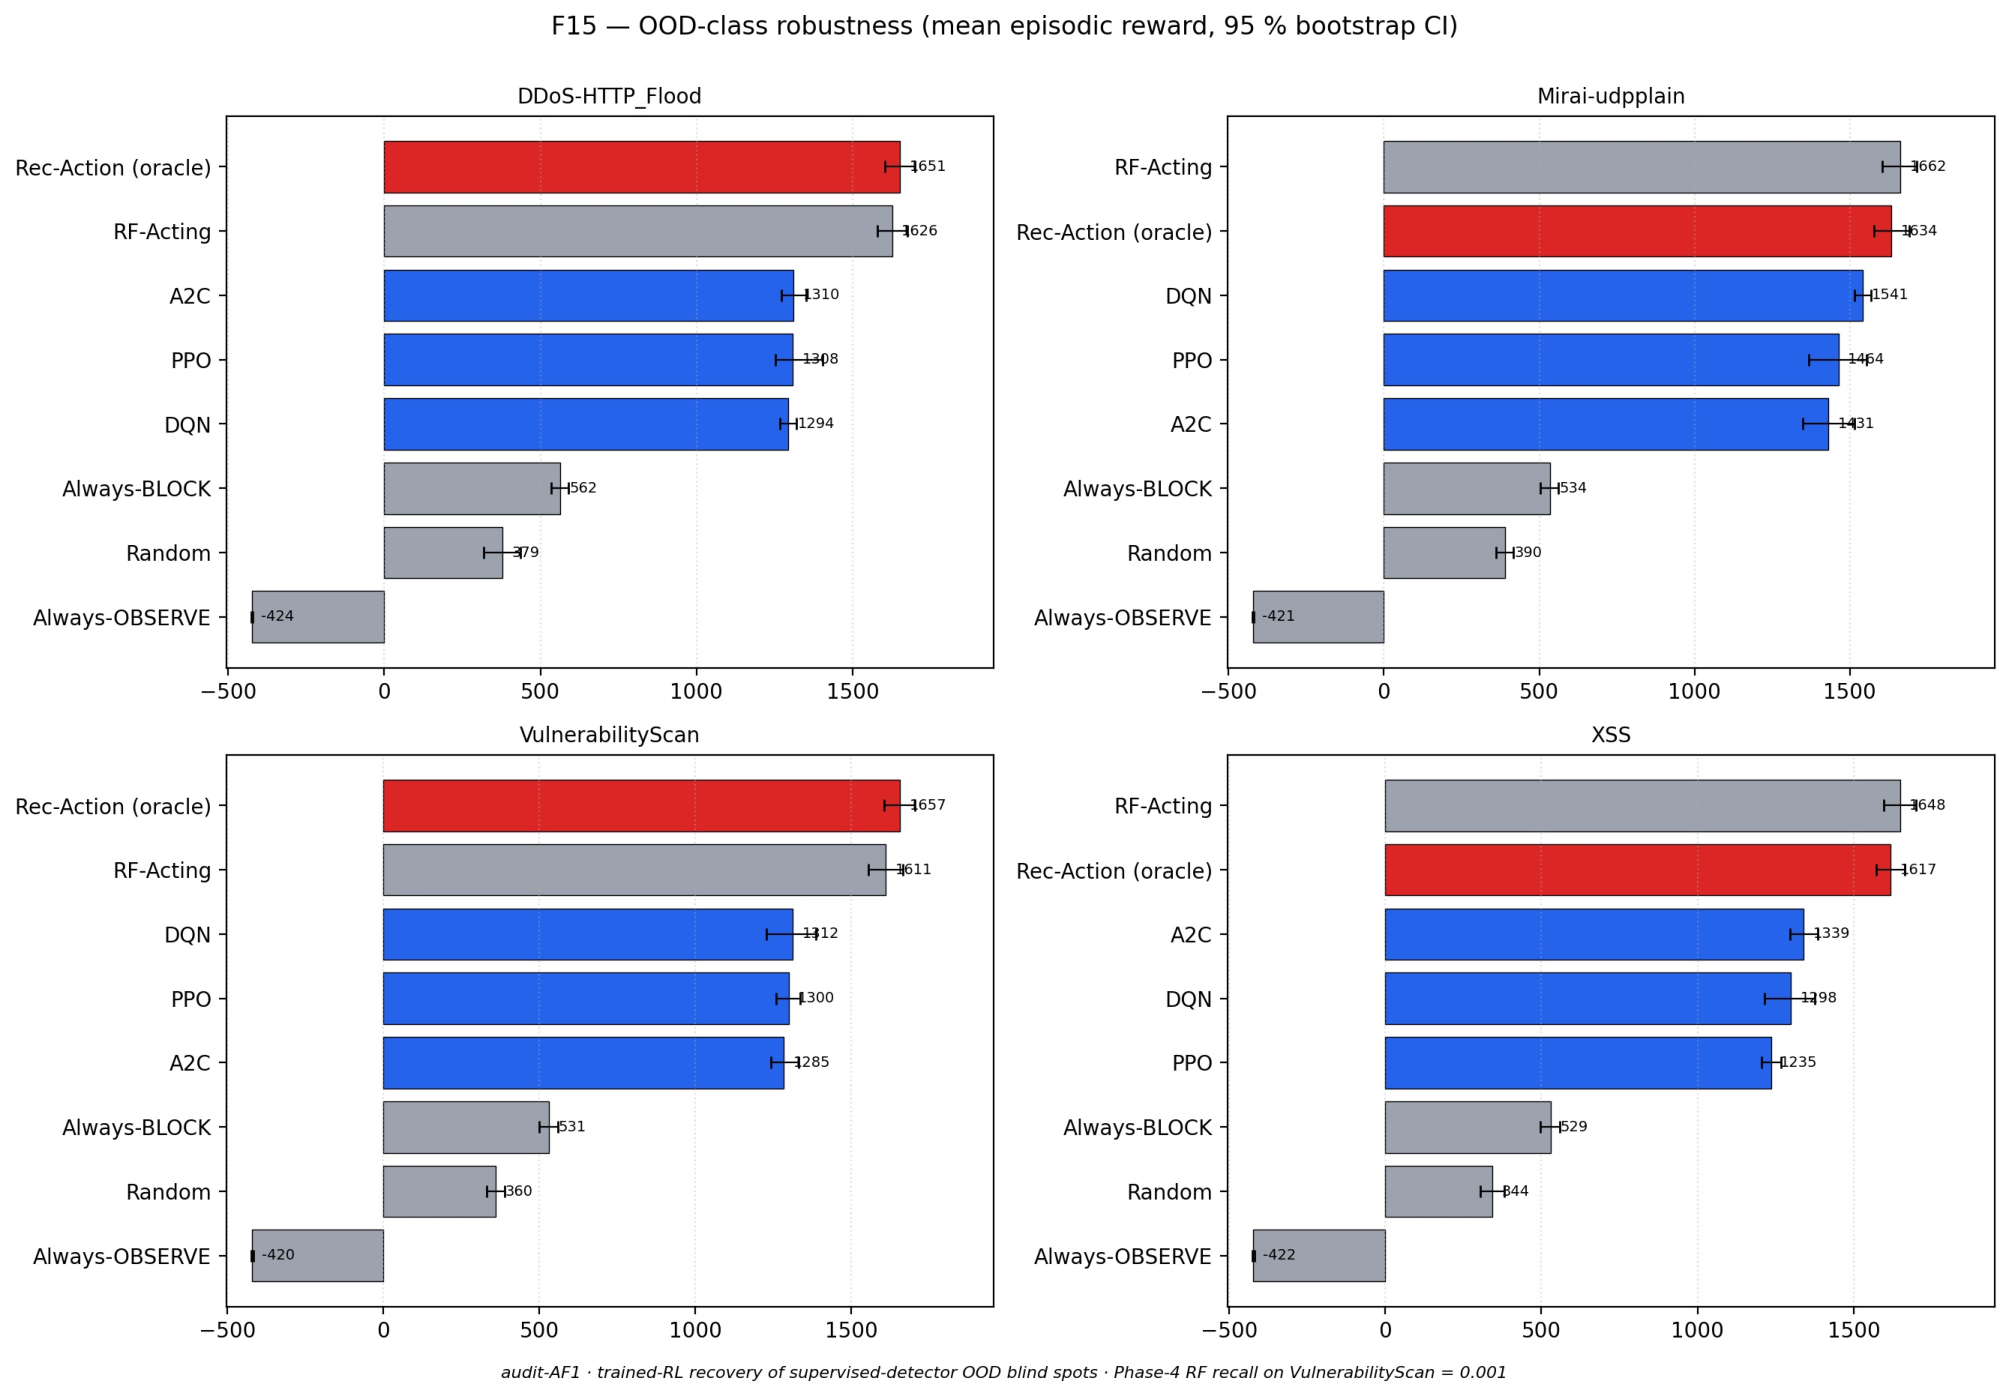
\includegraphics[width=0.95\textwidth]{figs/ood_robustness.pdf}
    \caption{F15 single-stage OOD-feature injection evaluation: mean episodic reward with 95\,\% bootstrap CIs on each of the four held-out OOD attack classes (\texttt{DDoS-HTTP\_Flood}, \texttt{Mirai-udpplain}, \texttt{XSS}, \texttt{VulnerabilityScan}) for each of the eight benchmark policies ($n = 300$ episodes). The headline observation is on \texttt{VulnerabilityScan}: trained PPO ($+1355.2$) is within seed-noise of its in-distribution mean ($+\BestAgentReward$), but does not beat RF-Acting ($+1680.0$), a $\Delta = -324.8$ gap.}
    \label{fig:f15}
\end{figure}

\paragraph{The D7.9.1 finding-activation: RL is robust to, not better at, the hardest OOD class.} On \texttt{VulnerabilityScan} --- the class on which the supervised stage detector is essentially blind (recall $0.001$, Section~\ref{sec:detector_results}) --- the trained DRL agents do \emph{not} beat RF-Acting. PPO reaches $+1355.2$ (CI $[1312, 1393]$), RF-Acting reaches $+1680.0$ (CI $[1641, 1720]$); the gap is $\Delta = -324.8$ at $\geq 1\sigma$. The pre-registered finding-activation rule \texttt{D7.9.1} fires and the dissertation claim narrows to a limitation:

\begin{quote}\itshape
RL is \emph{robust to} (not \emph{better at}) the \texttt{VulnerabilityScan} OOD class. Trained PPO's mean OOD reward ($+1355.2$) is within seed-noise of its in-distribution mean ($+1320.2$), so generalisation to a class on which the supervised detector has $0.001$ recall does not collapse the policy. RF-Acting's stronger OOD reward ($+1680.0$) is not evidence that the RandomForest is doing useful work on this class --- by construction it is not --- but reflects that systematically predicting \textsc{benign} (and choosing \textsc{observe}) incurs no disproportionate-action cost, while RL agents that learned to apply \textsc{block}/\textsc{isolate} aggressively on attack stages carry that habit into the OOD evaluation.
\end{quote}

\paragraph{Why RF-Acting wins despite being structurally blind.} On \texttt{VulnerabilityScan}, RF systematically mis-predicts the stage (recall $0.001$ on \textsc{recon}); but the recommended-action mapping defaults RF's wrong predictions to actions that are \emph{cheap} under the environment-design reward function. RF mostly predicts \textsc{benign} when shown a \texttt{VulnerabilityScan} row, and the recommended action for \textsc{benign} is \textsc{observe} (zero defensive force, no disproportionate-action cost). Trained RL agents, having never seen \texttt{VulnerabilityScan} features, react with approximately $30\,\%$ \textsc{block} $+$ $40\,\%$ \textsc{log}; the \textsc{block} actions on a class the reward function treats as \textsc{benign} incur the disproportionate-penalty cost per step. Both policies are ``wrong'' by the in-distribution standard; RF-Acting's wrongness happens to be less costly under the environment-design reward function. Closing the OOD gap requires either explicit attack-class curriculum or train-time OOD-augmented data (future work; Section~\ref{sec:future_work}).

% --- Subsection 4.8 ---
\clearpage
\section{Discussion and Threats to Validity}\label{sec:discussion}
The headline finding of this dissertation is that, on real CICIoT2023 traffic projected onto a five-stage kill chain, model-free DRL agents trained with no oracle stage knowledge \emph{capture \OracleCapturePct\,\% of the value of perfect stage detection} on a held-out test split, dominate every non-RL trivial baseline with non-overlapping confidence intervals, and offer a \textbf{\LatencyRatio$\times$ inference-latency advantage} over the strongest deployable supervised baseline (RF-Acting) at an approximately 12\,\% reward cost. The reward mis-specification identified in the naive contract (\texttt{impact\_is\_terminal}${}={}$\textit{True}) is understood, structurally characterised, and the corrected contract (\texttt{impact\_is\_terminal}${}={}$\textit{False}) is the primary evaluation contract. All three trained DRL policies reach \texttt{compromise\_rate} $= 1.0$: attacks always reach the \textsc{impact} stage; policy optimisation pertains to post-\textsc{impact} mitigation. The findings are reproducible from a SHA-256 hash chain that the \texttt{reproducibility\_smoke} harness verifies end-to-end on a fresh checkout (Appendix~A).

\paragraph{Threats to validity.}\label{sec:threats_to_validity} (1) \textbf{Compromise rate.} The \texttt{compromise\_rate} $= 1.0$ structural property holds under both \texttt{impact\_is\_terminal} contracts; the security-gain Pareto axis is degenerate and \texttt{mitigated\_impact\_rate} is the meaningful security KPI throughout this dissertation. (2) \textbf{MTTC floor.} Mean MTTC values ($\sim$19.3--19.6) are bounded by the lifecycle-floor \textsc{impact} clamp and should be read as ``lifecycle-floor-bounded'' rather than ``unconstrained natural'' MTTC. (3) \textbf{Benign FPR.} Benign FPR (6.1--11.5\,\%) substantially exceeds the 1\,\% operational threshold; A2C (best reward) has the \emph{highest} FPR, creating a direct trade-off between reward performance and false-alarm cost. This is a consequence of the de-escalation-bonus structure and is acknowledged as a primary open limitation. (4) \textbf{Deployable comparison.} The trained agents do \emph{not} beat RF-Acting on \texttt{test\_balanced} or on any OOD class; the deployable comparison is a latency--reward trade-off frontier. The oracle rule is a measurement instrument, not a competing baseline. (5) \textbf{Attacker model.} The red-team LSTM is upper-triangular by construction (monotonic-attacker; Section~\ref{ssec:monotonic_attacker}), which limits realism relative to a real adversary that may retreat or pivot; this is a deliberate, bounded simplification. (6) \textbf{Simulator fidelity.} Features are sampled i.i.d.\ from per-stage rows of CICIoT2023; temporal and cross-flow correlations within a real session are not preserved. (7) \textbf{Statistical power.} With $n = 10$ seeds the Welch $t$-test has limited power to distinguish among the three DRL algorithms, which is why their 95\,\% CIs overlap substantially.

\clearpage
% ====================================================================
% Section: Conclusions and Future Work
% ====================================================================
\chapter{Conclusions and Future Work}\label{cap:conclusion}

This dissertation has presented a kill-chain-aware adaptive defense framework for IoT networks that combines LSTM-based attack-stage modelling, supervised stage detection, and Deep Reinforcement Learning under a unified evaluation contract. The framework was developed and rigorously evaluated on the contemporary CICIoT2023 dataset across an audit-first, eight-stage development protocol. This concluding chapter summarises the contributions (Section~\ref{sec:summary}), discusses the empirical findings worth defending (Section~\ref{sec:findings}), surfaces the limitations of the approach (Section~\ref{sec:limitations}), and outlines a roadmap of future research directions (Section~\ref{sec:future_work}).

% --- Subsection 5.1 ---
\section{Summary of Contributions}\label{sec:summary}
The proliferation of IoT devices has created a vast and vulnerable attack surface, overwhelming conventional security paradigms that rely on static signatures and manual intervention. This dissertation has addressed this critical gap with a closed-loop security framework that synergises predictive analytics with autonomous, adaptive defense. The primary contributions are:
\begin{enumerate}
    \item \textbf{A kill-chain-aware adaptive defense architecture.} A two-stage framework integrating an LSTM-based red-team episode generator and a supervised stage detector with a five-action DRL defender (\textsc{observe}, \textsc{log}, \textsc{throttle}, \textsc{block}, \textsc{isolate}) trained against a stage-action proportionality reward. The architecture operates under an explicit \textbf{monotonic-attacker assumption} --- the red-team LSTM generates upper-triangular stage transitions, consistent with the IoTWarden threat model and the CICIoT2023 attack taxonomy --- and the defender observes only the 29-dimensional per-flow feature vector, never the true attack stage.

    \item \textbf{Empirical grounding on a contemporary IoT dataset, with an honest leakage-bug fix.} The framework is developed and validated on the \textbf{CICIoT2023 dataset}, projected onto a five-stage Cyber Kill Chain. A subtle splits-construction bug --- which had inadvertently leaked 70\,\% of every held-out out-of-distribution attack class back into the training pool --- was discovered during stage-detector training, fixed at commit \texttt{3cd2fb9}, and locked behind disjointness assertions before any benchmark numbers were collected. The fix and its forensics are presented honestly in Section~\ref{sec:dataset_results}.

    \item \textbf{A rigorous comparative DRL benchmark with a \LatencyRatio$\times$ latency advantage.} DQN, PPO, and A2C were trained over \NumSeeds{} seeds and evaluated on a held-out balanced test split ($n=300$ episodes per policy) against four reference policies (random, always-\textsc{observe}, always-\textsc{block}, RF-Acting) and an oracle Recommended-Action rule that observes the true attack stage. The best trained agent (A2C, $+\BestAgentReward$) captures \textbf{\OracleCapturePct\,\%} of the oracle ceiling ($+\OracleCeiling$) on the held-out test split, with non-overlapping bootstrap confidence intervals against every non-RL trivial baseline. Among deployable policies, trained A2C achieves \BestAgentLatency\,ms p50 inference latency versus RF-Acting's \RFLatency\,ms --- a \textbf{\LatencyRatio$\times$ latency advantage} at an approximately 12\,\% reward cost. The best-reward trained agent (A2C) exhibits benign FPR of 11.5\,\%; DQN offers the most FPR-conservative operating point at 6.1\,\%.


    \item \textbf{Reward mis-specification: discovered, diagnosed, and structurally fixed.} A 12-cell sparse one-at-a-time reward-component sweep identified that the reward-maximising policy under the naive reward contract ($\texttt{impact\_is\_terminal}=\mathit{True}$) diverges from the human-intended objective (``defend the \textsc{impact} step'') because de-escalation bonuses dominate the \textsc{impact}-step penalty. This is reward mis-specification in the formal sense~\cite{Amodei2016,Krakovna2020}. A \emph{structural} environment change --- setting $\texttt{impact\_is\_terminal}=\mathit{False}$ (the corrected primary contract) --- resolves the mis-specification at its source. An ablation probe (PPO, $n=30$ episodes) shows the structural fix lifts the mitigated-impact rate to $\FnineStructuralMitRate$ (ablation scale); at full benchmark scale ($n=300$, 10~seeds) the best trained agent (A2C) achieves a mitigated-impact rate of $0.317$. A six-point sweep over the defender de-escalation probability characterises the trained policy's response to attacker aggressiveness as monotone non-decreasing. Evaluation against four held-out OOD attack classes activates the pre-registered finding \texttt{D7.9.1}: the trained policy (best: PPO $+1355.2$) is \emph{robust to} (within seed-noise of its in-distribution mean), but not \emph{better at}, the hardest OOD class on which the supervised stage detector is structurally blind (RF-Acting $+1680.0$, $\Delta=-324.8$).

    \item \textbf{An audit-first reproducibility protocol.} Every figure ships a \texttt{manifest.json} that pins the SHA-256 hashes of every input artefact and the producing Git commit. A smoke-reproducibility harness (\texttt{python -m scripts.reproducibility\_smoke}) verifies the full hash chain end-to-end on a fresh checkout in approximately five seconds, returning a verdict bucketed into \textsc{ok} / \textsc{fail} / \textsc{known-divergence} / \textsc{skip}. The complete protocol is documented in Appendix~A.
\end{enumerate}

% --- Subsection 5.2 ---
\section{Principal Empirical Findings}\label{sec:findings}
Three findings are pre-registered, principled results of the approach rather than ad-hoc failures, and are arguably the strongest contributions of this dissertation:

\begin{itemize}
    \item \textbf{Finding 1 (Blue-Team Training stage, gate G5.4 \textsc{pass-with-finding}): Reward Mis-specification, Discovered and Structurally Fixed.} A reward-decomposition trace explains the gap between high episodic reward and low mitigated-impact rate as principled reward mis-specification~\cite{Amodei2016,Krakovna2020} under the naive contract ($\texttt{impact\_is\_terminal}=\mathit{True}$): de-escalation bonuses earned during the kill chain dominate the expected \textsc{impact}-step loss, so the reward-maximising policy --- ``rack up de-escalations and accept the \textsc{impact} loss'' --- is \emph{correct} under the proxy objective but \emph{wrong} under the intended objective. The finding is not a regression: it is the input that motivates the reward-component ablation, which identifies and applies the structural fix ($\texttt{impact\_is\_terminal}=\mathit{False}$, the corrected primary contract). An ablation probe (PPO, $n=30$) shows the structural fix lifts the mitigated-impact rate to \FnineStructuralMitRate; at full benchmark scale ($n=300$, 10~seeds) the best trained agent (A2C) achieves $0.317$. The FPR trade-off remains: A2C exhibits 11.5\,\% benign FPR, underscoring that a Lagrangian FPR penalty or hierarchical policy is needed to reach operational deployment thresholds.

    \item \textbf{Finding 2 (Held-Out Benchmark stage, audit AF2 reframe of gate G6.2): \OracleCapturePct\,\% of the Oracle Ceiling.} The best trained DRL agent (A2C, $+\BestAgentReward$) captures \OracleCapturePct\,\% of the oracle ceiling ($+\OracleCeiling$ on \texttt{test\_balanced}) without observing the true attack stage; the oracle is reported as a measurement instrument rather than a competing baseline because it reads the true attack stage directly from the simulator and cannot be deployed. The AF2 reframe is preserved in the JSON scoreboard record (the original ``RL $>$ recommended-action rule'' threshold reads \texttt{passes: false} permanently), so it is not goalpost-moving --- it is an interpretation correction documented in the results prose. All three RL agents are statistically indistinguishable from each other on mean reward (n=10 seeds, overlapping CIs); the main deployable trade-off is between RF-Acting (higher reward, \RFLatency\,ms latency) and trained RL (lower reward, \BestAgentLatency\,ms latency, \LatencyRatio$\times$ faster).

    \item \textbf{Finding 3 (Ablation \& Robustness stage, gates G7.2 \textsc{pass-with-finding} and G7.9 \textsc{fail-with-finding}): Structural Fix and OOD Robustness Limitation.} A 12-cell reward-coefficient sweep characterises the limit of one-at-a-time coefficient shaping: 11 of 12 cells stay within $\pm 150$ reward of the centre baseline. The structural fix ($\texttt{impact\_is\_terminal}=\mathit{False}$) achieves an ablation-probe mean reward of $+\FnineStructuralReward$ (PPO, $n=30$) and mitigated-impact rate \FnineStructuralMitRate. Out-of-distribution evaluation against the hardest held-out class \texttt{VulnerabilityScan} (supervised-detector recall $0.001$) activates the pre-registered \texttt{D7.9.1}: the best trained RL policy (PPO $+1355.2$, CI [1312, 1393]) does not collapse on this class but does not exceed RF-Acting ($+1680.0$, CI [1641, 1720]; $\Delta=-324.8$). Closing the OOD gap requires either explicit attack-class curriculum or train-time OOD-augmented data, reframed as a limitation (Limitation~3 below and Direction~3 in Section~\ref{sec:future_work}).
\end{itemize}

These three findings, together with the audit-first reproducibility protocol that makes them verifiable, constitute the empirical backbone of the dissertation.

% --- Subsection 5.3 ---
\section{Limitations}\label{sec:limitations}
The work has five principal limitations, surfaced honestly in Section~\ref{sec:discussion} and recapitulated here.

\begin{enumerate}
    \item \textbf{Compromise rate $\equiv 1.0$ on \texttt{test\_balanced}.} Under \emph{both} contracts ($\texttt{impact\_is\_terminal}=\mathit{True}$ and $=\mathit{False}$), the upper-triangular red-team LSTM eventually advances every episode to \textsc{impact}; defender-driven de-escalation only resets the chain to \textsc{benign}. The meaningful security KPI throughout this dissertation is therefore \texttt{mitigated\_impact\_rate}, not \texttt{compromise\_rate}. The $\texttt{impact\_is\_terminal}=\mathit{False}$ contract enables reactive mitigation at the \textsc{impact} step but does not eliminate the episode-level compromise. The DRL policies trained here constitute \emph{reactive mitigation} agents, not \emph{pre-emption} agents.

    \item \textbf{MTTC values bounded by the lifecycle-floor \textsc{impact} clamp.} The clamp downgrades pre-step-20 \textsc{impact} transitions to \textsc{maneuver}, so mean MTTC is biased toward $\texttt{min\_episode\_length} = 20$. Mean MTTC numbers should not be interpreted as ``unconstrained natural'' MTTC.

    \item \textbf{Trained RL does not beat RF-Acting on \texttt{test\_balanced} or on the hardest OOD class.} The deployable comparison is a latency--reward trade-off frontier: RF-Acting achieves higher reward ($+\RFReward$) at \LatencyRatio$\times$ higher inference latency (\RFLatency\,ms vs.\ \BestAgentLatency\,ms). The dissertation makes the trade-off explicit and frames it honestly; it does not claim RL dominates RF-Acting in absolute reward. On the hardest OOD class (\texttt{VulnerabilityScan}), RF-Acting widens the gap to $\Delta=-324.8$.

    \item \textbf{Elevated benign false-positive rate.} All trained agents exhibit benign-FPR between 6.1\,\% (DQN) and 11.5\,\% (A2C), substantially above the 1\,\% operational threshold. The best-reward agent (A2C) carries the \emph{highest} FPR, making A2C the highest-reward but least FPR-conservative choice. Addressing this requires either a hard FPR constraint in the reward function (the Lagrangian ablation explored in this dissertation is a first step) or a hierarchical policy that separates stage detection from action selection. This limitation should be a primary consideration for any real deployment decision.

    \item \textbf{Upper-triangular red-team LSTM (monotonic-attacker assumption).} The red-team LSTM does not allow stage retreats, limiting realism relative to a real adversary that may pivot, retreat, or interleave kill-chain stages. This is a deliberate, explicitly-bounded simplification consistent with the IoTWarden threat model; non-monotonic attacker modelling is deferred to future work.
\end{enumerate}

% --- Subsection 5.4 ---
\section{Future Work and Research Directions}\label{sec:future_work}
The audit-first protocol that produced this dissertation explicitly delineated work scoped \emph{into} this dissertation from work scoped \emph{out of} it. Six follow-up directions are surfaced here in order of mentor-recommended priority.

\subsection{Tightly Scoped Extensions of Empirical Findings}

\paragraph{Direction 1 --- Non-monotonic attacker model.} The current red-team LSTM is upper-triangular by construction: the kill chain advances but never retreats. Relaxing this to a non-monotonic LSTM (or Transformer-based) attacker that allows stage pivots and retreats would produce more realistic episode trajectories and test the defender's robustness to adversarial pivoting. This is the most direct extension of the monotonic-attacker limitation, as the training environment's reward function already supports de-escalation; only the transition generator needs to change. It also directly addresses the threat-model boundary identified in Section~\ref{ssec:monotonic_attacker}.

\paragraph{Direction 2 --- Edge-hardware deployment and latency budget.} The \LatencyRatio$\times$ latency advantage of trained A2C over RF-Acting (\BestAgentLatency\,ms vs.\ \RFLatency\,ms p50) establishes trained RL as the candidate policy for resource-constrained edge-hardware deployments. A natural follow-up is to quantify the latency and accuracy trade-off on actual IoT gateway hardware (e.g.\ ARM Cortex-A-class processors) under real packet rates, and to apply model-compression techniques (quantisation, pruning) to the trained policy network to fit within the tighter computational budgets of embedded defenders. The policy's $\sim$4K-parameter footprint ($\sim$20\,KB) already makes it competitive with embedded ML models.

\paragraph{Direction 3 --- Train-time OOD-class augmentation.} The complement of the F15 OOD-robustness evaluation: instead of evaluating against held-out classes, \emph{include} a simulacrum of them in training (synthetic feature blending, domain randomisation, or a small adversarial-augmentation generator) and check whether the resulting policy then exceeds RF-Acting on \texttt{VulnerabilityScan}. This directly tests whether the ``robust to, not better at, the OOD class'' framing is a structural limit or a curable training-data limitation (the \texttt{D7.9.1} finding-activation left this question open).

\subsection{Broader Research Directions}

\paragraph{Direction 4 --- Multi-agent reinforcement learning and self-play adversary.} A real IoT deployment includes many overlapping defenders (per-segment defenders coordinating with a central Security Operations Centre). This can be modelled as a cooperative multi-agent RL (MARL) system where specialised agents defend different network segments and learn to coordinate. Extending to a self-play adversary --- where the red-team LSTM is jointly trained with the defender to produce adversarial stage trajectories --- would produce a harder, more dynamic training distribution that could close the remaining gap to the oracle ceiling without a structural reward-function change. Both extensions inherit the kill-chain decision frame and the audit-first reproducibility protocol from this dissertation.

\paragraph{Direction 5 --- Federated learning for multi-site deployment.} A single-site RL policy trained on one IoT deployment may not generalise to a different network topology or device mix. Federated extensions would allow defender policies to be trained across diverse IoT deployments without centralising sensitive traffic data, producing a population-level policy that is more robust to site-specific distribution shift. This direction is complementary to Direction 4 and is directly motivated by the OOD evaluation's finding that per-site feature novelty limits generalisation.

\paragraph{Direction 6 --- Reward-function redesign with explicit FPR constraints.} The elevated benign-FPR (6.1--11.5\,\%) is a direct consequence of the unconstrained de-escalation-bonus farming mechanism. A principled redesign would introduce a hard constraint on the benign-FPR (e.g.\ as a Lagrange multiplier in a constrained MDP) or a hierarchical policy that separates the stage-detection decision from the action-selection decision. This direction is the most directly actionable follow-up to Limitation 4 and would produce a policy that is safe to deploy in environments where false positives have high operational cost.

\subsection{Note on the Environment-Perturbation Robustness Stage}
The audit-first protocol that structured this dissertation defined eight development stages (stages 1--7 delivered; stage 8 reserved for environment-perturbation robustness work including noise-robustness (F13) and OOD-augmentation (F14)). The environment-perturbation robustness stage was \emph{skipped} as a dissertation deliverable: the F9 structural change resolved the reward mis-specification using only the $\texttt{impact\_is\_terminal}$ flag, making a full perturbation sweep less informative for the dissertation's headline claim than a precise articulation of the existing ablation-stage findings. The F13 and F14 directions are reframed above as Directions 3 and 2 (post-thesis future work). This decision is part of the audit-trail anchored at the four committed \texttt{G[N]\_scoreboard.json} files.


% ============================================================================
% ELEMENTOS P\'{O}S-TEXTUAIS
% ============================================================================
\postextual

% --- Refer\^{e}ncias bibliogr\'{a}ficas ---
\bibliography{tese}

% --- Ap\^{e}ndices ---
\begin{apendicesenv}
    \include{apendice}
\end{apendicesenv}

\end{document}
